\documentclass[10pt,a4paper]{report}
\usepackage[utf8]{inputenc}
\usepackage[russian]{babel}
\usepackage[OT1]{fontenc}
\usepackage{amsmath}
\usepackage{amsfonts}
\usepackage{amssymb}
\usepackage{graphicx}
\author{Скрипаль Борис, Баратынский Александр}
\title{Отчет по лабораторной работе по дисциплине "Сети и системы передачи данных"\newline
на тему "Визуализация сигналов во временной и частотной области"}
\date{23.02.14}
\begin{document}
\maketitle
\pagebreak
\chapter{Лабораторная работа 4}
\section{Цель работы}
Познакомиться со средствами генерации сигналов и визуализации их спектров.
\section{Постановка задачи}
В командном окне MATLAB и в среде Simulink промоделировать чистый синусоидальный сигнал, 
так же синусоидальный сигнал с шумом. Получить их спектры.
\section{Введение}
В ходе данной лабораторной работы необходимо промоделировать чистый синусоидальный сигнал, а так же синусоидальный сигнал с шумом и получить их представления во временной и частотной областях. Синусоидальный сигнал задаётся по следующей формуле: 
\begin{displaymath}
A(t) = A_0 * sin(2*\pi *f*t + u_0)
\end{displaymath}
Для создания зашумленного синусоидального сигнала, к чистому синусоидальному сигналу прибавляется случайная составляющая, по формуле:
\begin{displaymath}
A(t) = A_0 * sin(2*\pi *f*t + u_0) + A_1*rand()
\end{displaymath}
Для выделения частот регулярных составляющих сигнала необходимо использовать преобразование Фурье, реализуемое следующей формулой:
\begin{displaymath}
X(k) = \sum_{j=1}^N x(j)*e^{2*\frac{x}{N(j-1)(k-1)}}
\end{displaymath}
\section{Алгоритм работы}
\begin{itemize}
\item Построение чистого синусоидального сигнала с регулярной составляющей 10 Гц и с нулевой начальной фазой
\item Вывод временной характеристики сигнала
\item Реализация одномерного преобразования Фурье на основе 512 точек
\item Построение графика спектральной плотности для чистого синусоидального сигнала
\item Построение зашумленного синусоидального сигнала путем добавления к чистому синусоидальному сигналу случайной аддитивной компоненты с нулевым средним
\item Вывод временной характеристики полученного сигнала
\item Реализазия одномерного преобразования Фурье на основе 512 точек
\item Построение графика спектральной плотности для зашумленного синусоидального сигнала
\end{itemize}
\section{Код MATLAB}
x = 0:0.01:4*pi;\newline
t0 = 10;\newline
\%исходный сигнал\newline
ynorm = sin(2*pi*t0*x);\newline
plot(x(1:200),ynorm(1:200))\newline
grid\newline
\%спектр исходного сигнала\newline
figure\newline
spectrum = fft(ynorm,512);\newline
normspectrum = spectrum.*conj(spectrum)/512;\newline
f=100*(0:255)/512;\newline
plot(f, normspectrum(1:256))\newline
axis([0 max(f) 0 10])\newline
grid\newline
\%зашумленный сигнал\newline
ynoize = ynorm+ 0.8*rand(size(x));\newline
figure\newline
plot(x(1:200),ynoize(1:200));\newline
grid\newline
\%спектр зашумленного сигнала\newline
spectrum = fft(ynoize,512);\newline
noizespectrum = spectrum.*conj(spectrum)/512;\newline
figure\newline
plot(f, noizespectrum(1:256))\newline
axis([0 max(f) 0 10])\newline
grid\newline
\section{Результаты работы}
В результате выполнения программы мы получили четыре графика: временная и частотная характеристика для чистого и зашумленного синусоидального сигнала. Графики представленны ниже. \newpage
\begin{figure}
\begin{center}
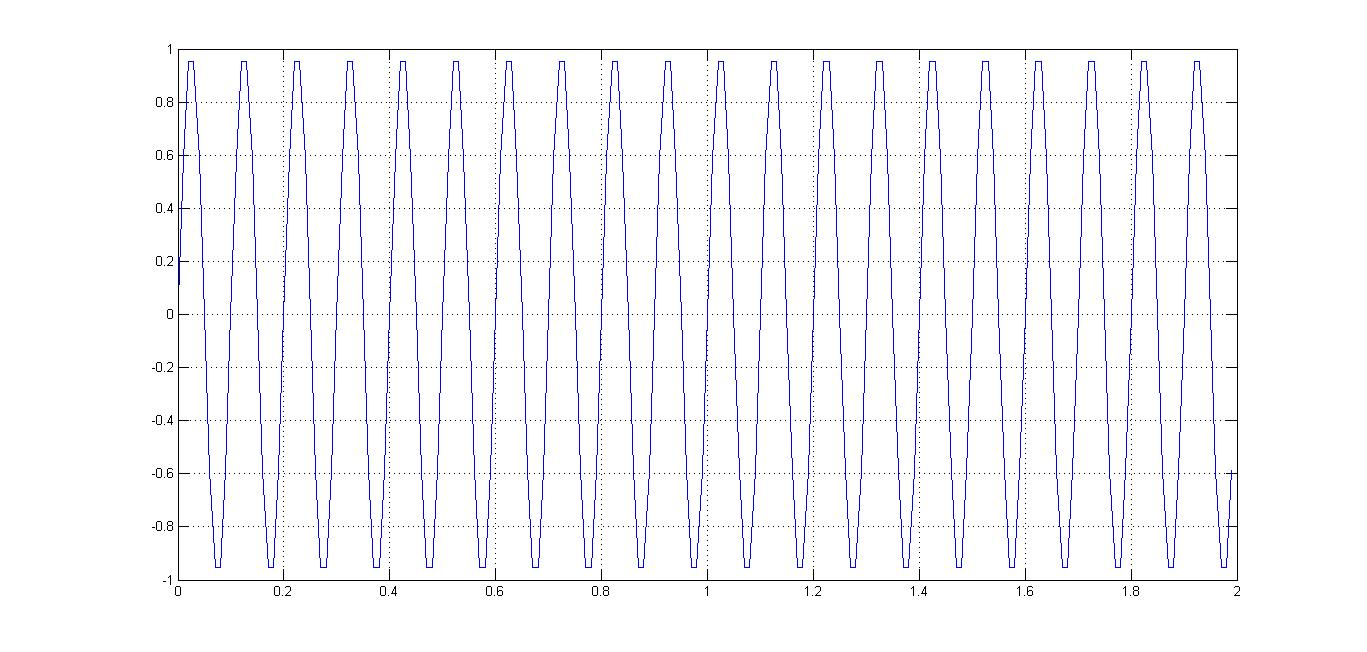
\includegraphics[width=150mm, scale = 0.3]{sint.jpg}
рис. 1 Временная характеристика чистого синусоидального сигнала
\end{center}
\begin{center}
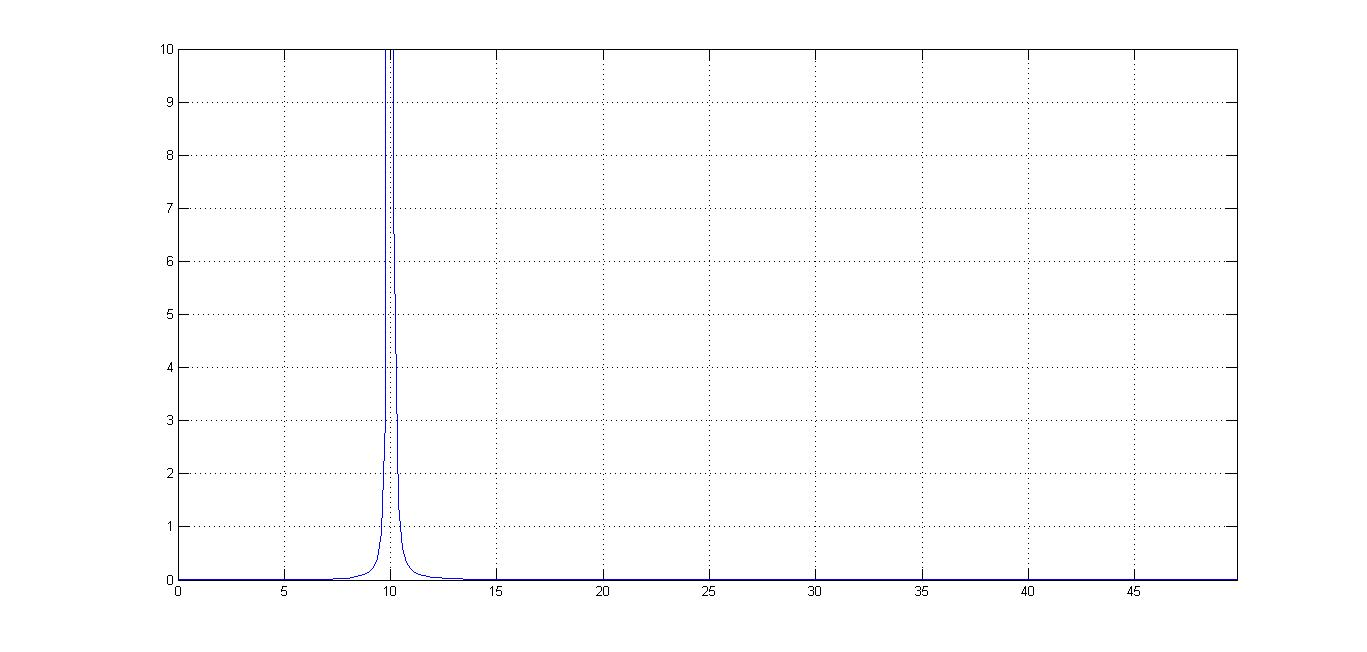
\includegraphics[width=150mm, scale = 0.3]{sinch.jpg}
\end{center}
рис. 2. Частотная характеристика чистого синусоидального сигнала
\end{figure}
\begin{figure}
\begin{center}
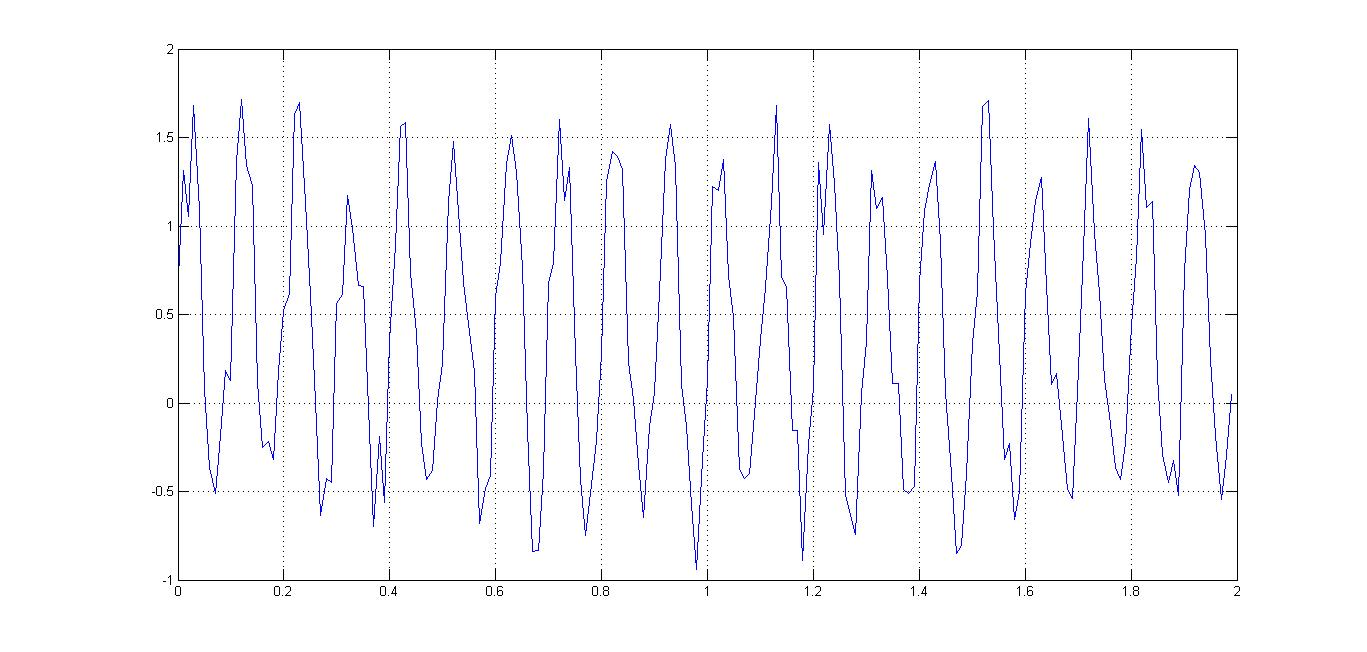
\includegraphics[width=150mm, scale = 0.3]{nsint.jpg}
\end{center}
рис. 3. Временная характеристика зашумленного синусоидального сигнала
\begin{center}
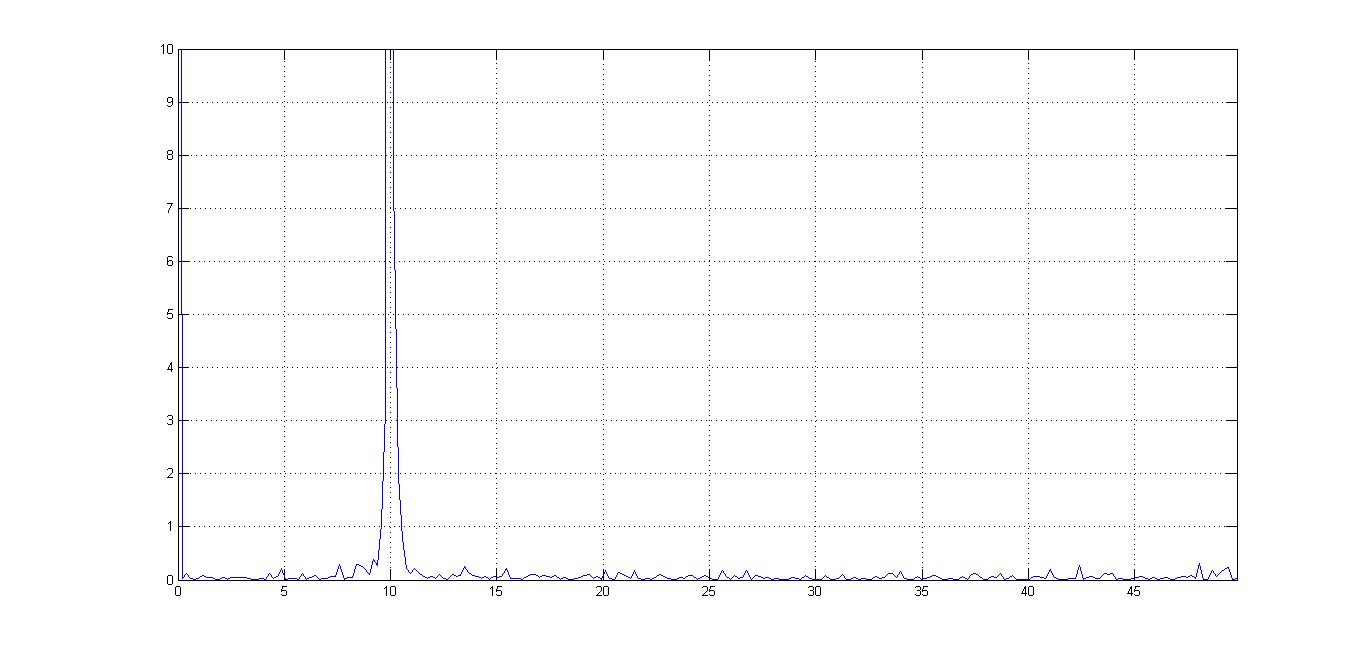
\includegraphics[width=150mm, scale = 0.3]{nsinch.jpg}
\end{center}
рис. 4. Частотная характеристика зашумленного синусоидального сигнала
\end{figure}
Как видно из графиков, регулярная составляющая, как у чистого синусоидальног осигнала, так и у зашумленного равна 10Гц. Временная же характеристика чистого и зашумленного сигнала отличается достаточно сильно, хотя в обоих случаях заметны общие черты.
\section{Вывод}
Данная лабораторная работа заключалась в получении и сравнении спектров чистого и зашумленного сигнала. Спектры сигналов вычислялись на ограниченном промежутке. Для этого длина промежутка и частота квантования выбирались так, чтобы результаты вычислений были достаточно точными. Полученные значения совпали с ожидаемыми. Стоит отметить, что спектр получается периодическим по частоте.

Теоретически , спектр синуса должен выглядеть как один импульс очень малой ширины.Но, из-за того, что синус конечный, то есть умноженный на прямоугольное окно, то и его спектр сворачивается со спектром прямоугольного окна. Так как наш сигнал дискретизирован, он умножается на решетку дельта-импульсов. Спектр решетки дельта-импульсов - также решетка дельта-импульсов, и спектр нашего сигнала сворачивается также с решеткой дельта-импульсов. Из-за чего получается спектр в виде нескольких импульсов.
\chapter{Лабораторная работа 5}
\section{Цель работы}
Целью данной работы является получение представлений о свойствах спектров, а именно:
\begin{itemize}
\item Построение полигармонического сигнала
\item Построение прямоугольного импульсного сигнала
\item Построение треугольного импульсного сигнала
\item Получение спектров этих сигналов
\item Создание моделей в Simulink
\end{itemize}
\section{Теоритическая часть}
В данной работе мы рассматриваем три типа сигналов: полигармонический, прямоугольный импульсный и треугольный. Их формулы представленны ниже:
\begin{itemize}
\item полигармонический сигнал 
\end{itemize}
\begin{displaymath}
y(t) = \sum_{n=0}^N-1 cos(nt)
\end{displaymath}
\begin{itemize}
\item прямоугольный импульсный сигнал
\end{itemize}
\begin{displaymath}
y(t) = \Pi (t,T_i)
\end{displaymath}
\begin{itemize}
\item треугольный импульсный сигнал
\end{itemize}
\begin{displaymath}
y(t) = \Delta (t,T_i)
\end{displaymath}
Для получения треугольного сигнала используется операция свертки двух прямоугольных сигналов, производимая по формуле:
\begin{displaymath}
(f*g)(x) = int_inf^-inf f(y)g(x-y)dy
\end{displaymath}
\section{Код matlab}
\begin{verbatim}
x = 0:0.01:4*pi;\newline
f0=5;\newline
y = 0;\newline
for i=0:1:100\newline
    y = y + cos(i*x);\newline
end \newline
plot(x(1:100),y(1:100))\newline
grid\newline
figure\newline
spectrum = fft(y,512);\newline
norm_spectrum = spectrum.*conj(spectrum)/512;\newline
f=100*(0:255)/512;\newline
plot(f, norm_spectrum(1:256))\newline
axis([0 max(f) 0 10])\newline
grid\newline
figure\newline
y1 = square(x,50);\newline
plot(x(1:1000),y1(1:1000),'LineWidth',2);\newline
ylim([-1.2,1.2]);\newline
grid\newline
figure\newline
spectrum = fft(y1,512);\newline
norm_spectrum = spectrum.*conj(spectrum)/512;\newline
f1=100*(0:255)/512;\newline
plot(f1, norm_spectrum(1:256))\newline
axis([0 max(f1) 0 10])\newline
grid\newline
figure\newline
y2 = conv(square(x,50),square(x,50));\newline
plot(x(1:1000),y2(1:1000),'LineWidth',2);\newline
grid\newline
figure\newline
spectrum = fft(y2,512);\newline
norm_spectrum = spectrum.*conj(spectrum)/512;\newline
f2=100*(0:255)/512;\newline
plot(f2, norm_spectrum(1:256)/1000)\newline
axis([0 max(f2) 0 50])\newline
grid\newline
\end{verbatim}
\section{Результаты работы}
В результате, были полученны 6 графиков: графики полигармонического, прямоугольного и треугольного сигналов, а так же графики их спектров соответственно. Графики представлены на рисунках ниже.
\begin{figure}
\begin{center}
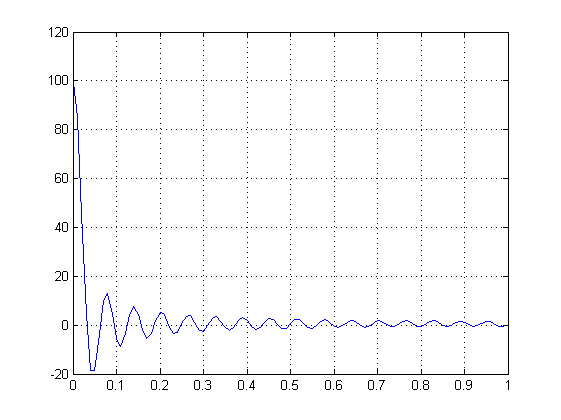
\includegraphics[width=150mm, scale = 0.9]{5_1.png}\newline
рис. 5. Полигармонический сигнал\newline
\end{center}
\end{figure}
\begin{figure}
\begin{center}
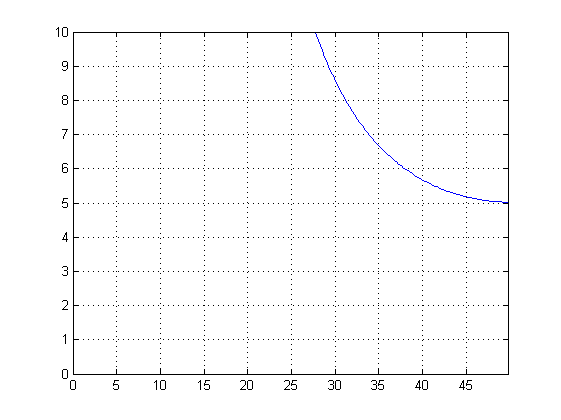
\includegraphics[width=150mm, scale = 0.9]{5_2.png}\newline
рис. 6. Спектр полигармонического сигнала\newline
\end{center}
\end{figure}
\begin{figure}
\begin{center}
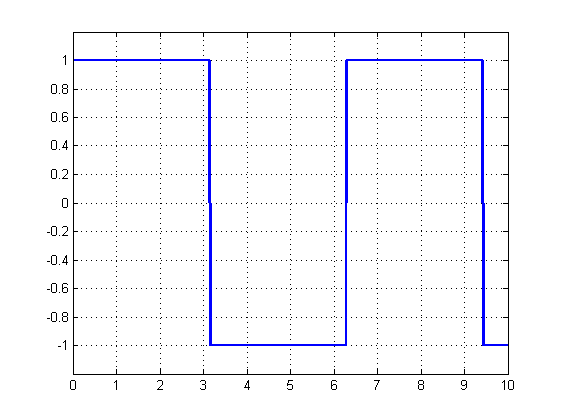
\includegraphics[width=150mm, scale = 0.9]{5_3.png}\newline
рис. 7. Прямоугольный сигнал\newline
\end{center}
\end{figure}
\begin{figure}
\begin{center}
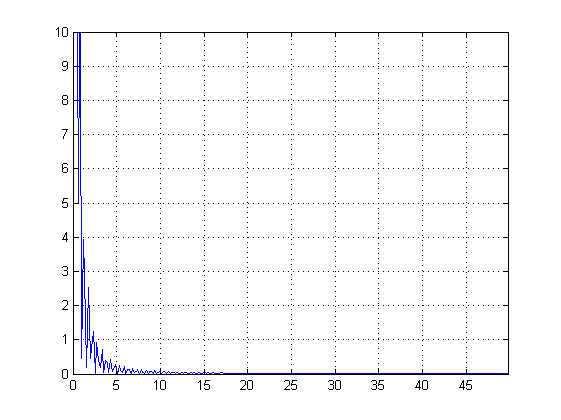
\includegraphics[width=150mm, scale = 0.9]{5_4.png}\newline
рис. 8. Спектр прямоугольного сигнала\newline
\end{center}
\end{figure}
\begin{figure}
\begin{center}
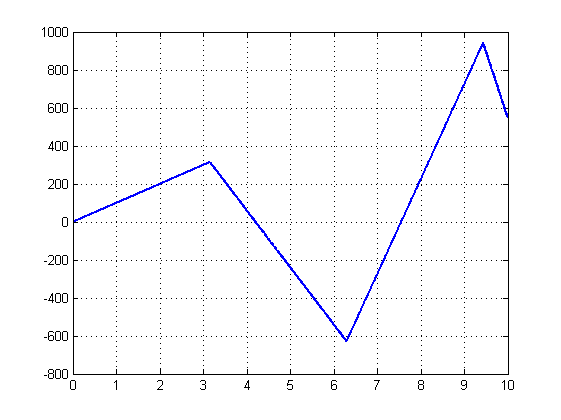
\includegraphics[width=150mm, scale = 0.9]{5_5.png}\newline
рис. 9. Треугольный сигнал\newline
\end{center}
\end{figure}
\begin{figure}
\begin{center}
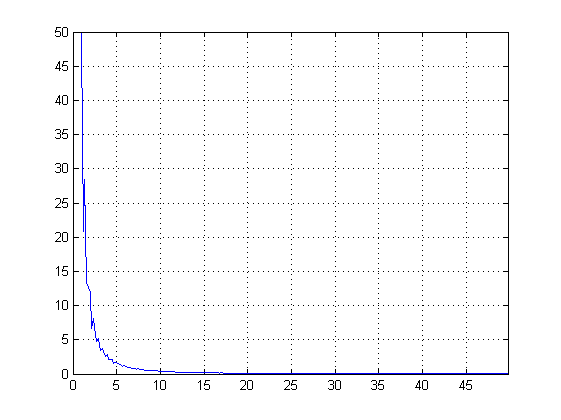
\includegraphics[width=150mm, scale = 0.9]{5_6.png}\newline
рис. 10. Спектр треугольного сигнала\newline
\end{center}
\end{figure}
Ниже представлены результаты работы в Simulink
\begin{figure}
\begin{center}
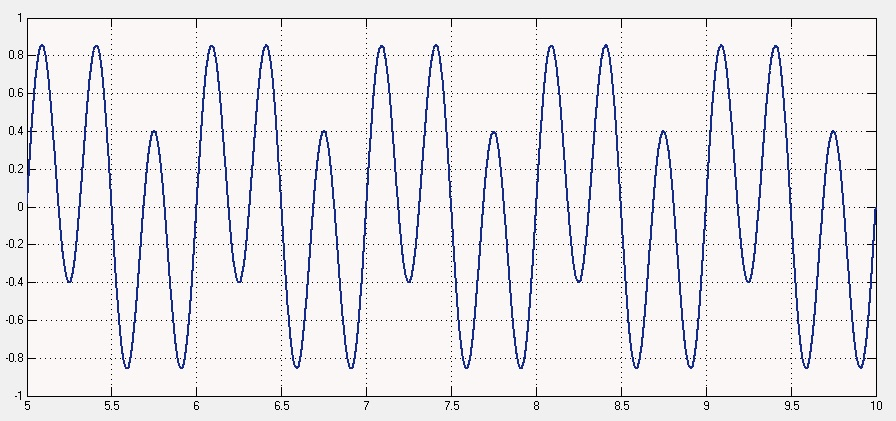
\includegraphics[width=150mm, scale = 0.9]{5_7.jpg}\newline
рис. 11. Полигармонический сигнал\newline
\end{center}
\end{figure}
\begin{figure}
\begin{center}
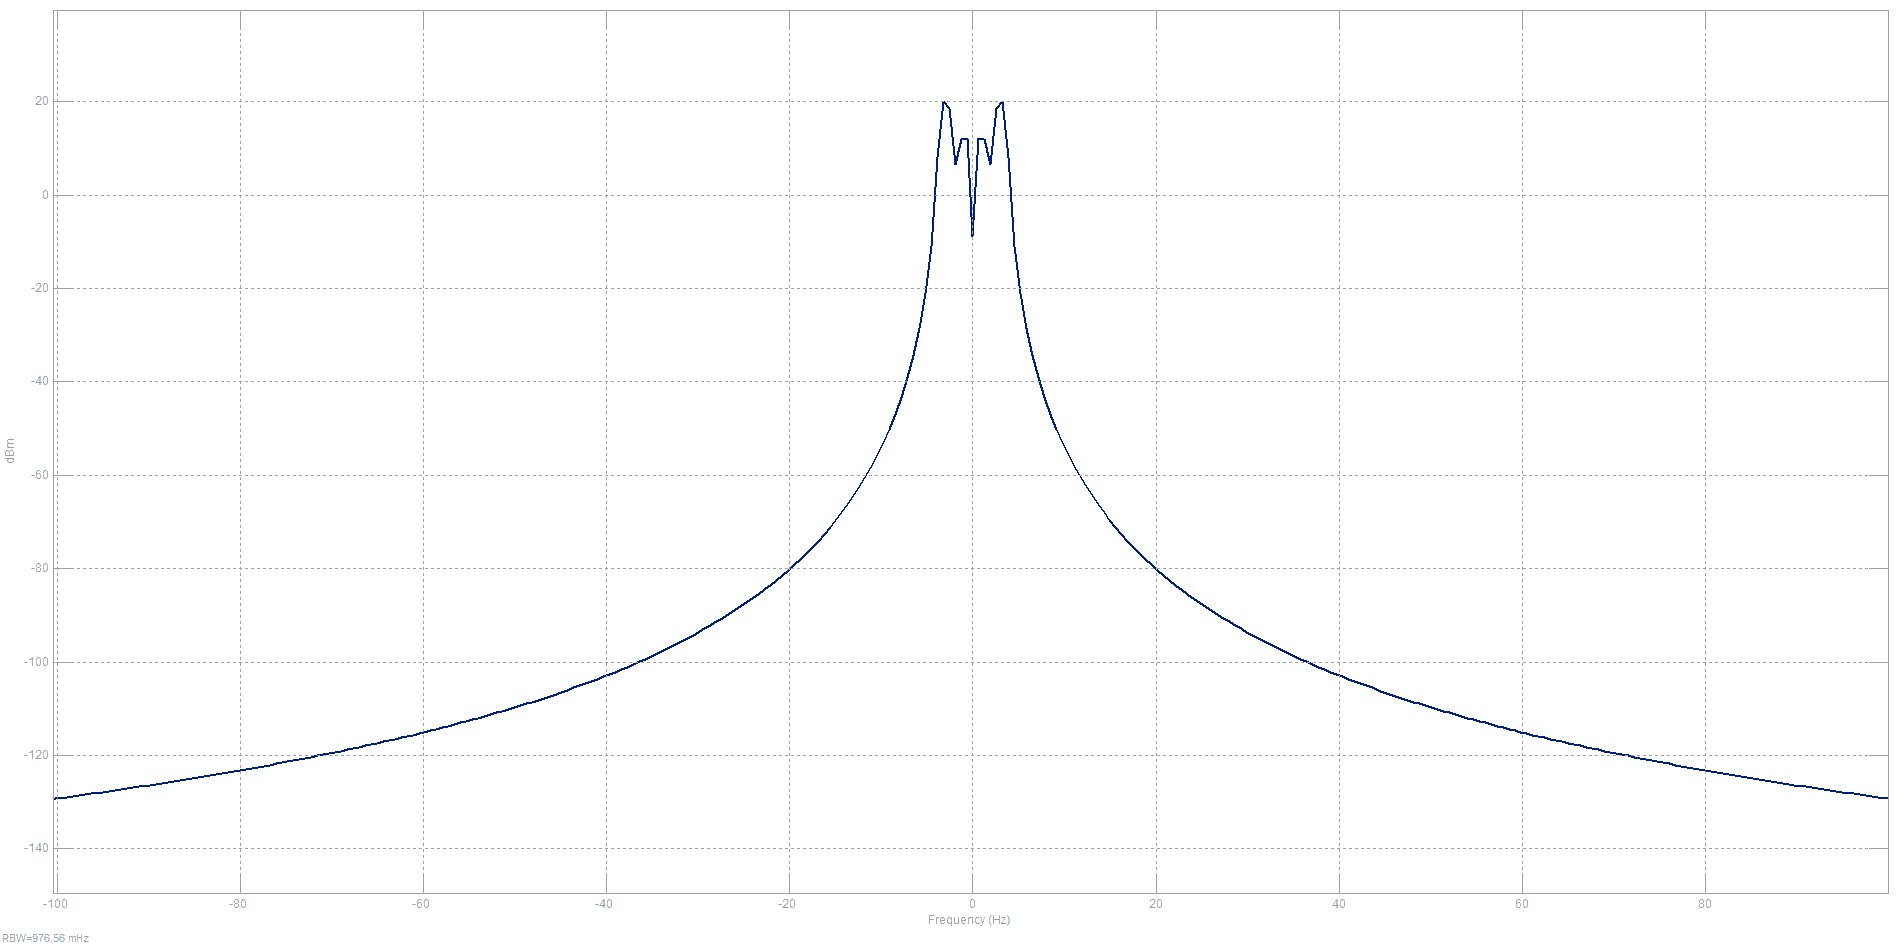
\includegraphics[width=150mm, scale = 0.9]{5_8.jpg}\newline
рис. 12. Спектр полигармонического сигнала\newline
\end{center}
\end{figure}
\begin{figure}
\begin{center}
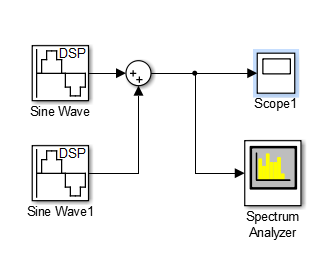
\includegraphics[width=150mm, scale = 0.9]{5_9.jpg}\newline
рис. 13. Модель\newline
\end{center}
\end{figure}
\begin{figure}
\begin{center}
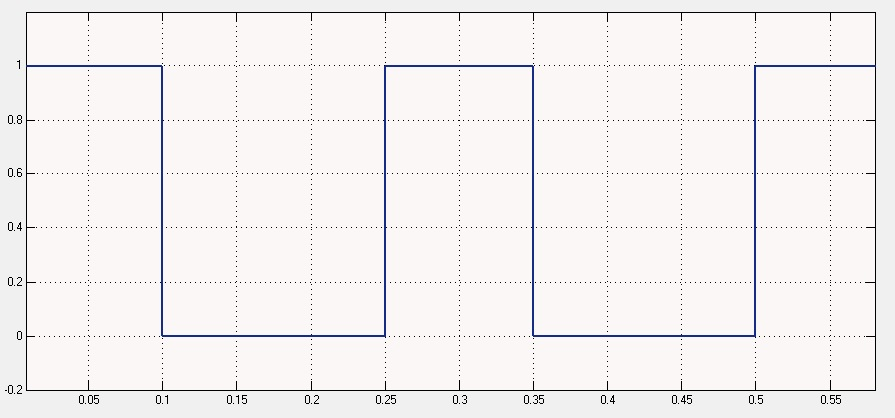
\includegraphics[width=150mm, scale = 0.9]{5_10.jpg}\newline
рис. 14. Прямоугольный сигнал\newline
\end{center}
\end{figure}
\begin{figure}
\begin{center}
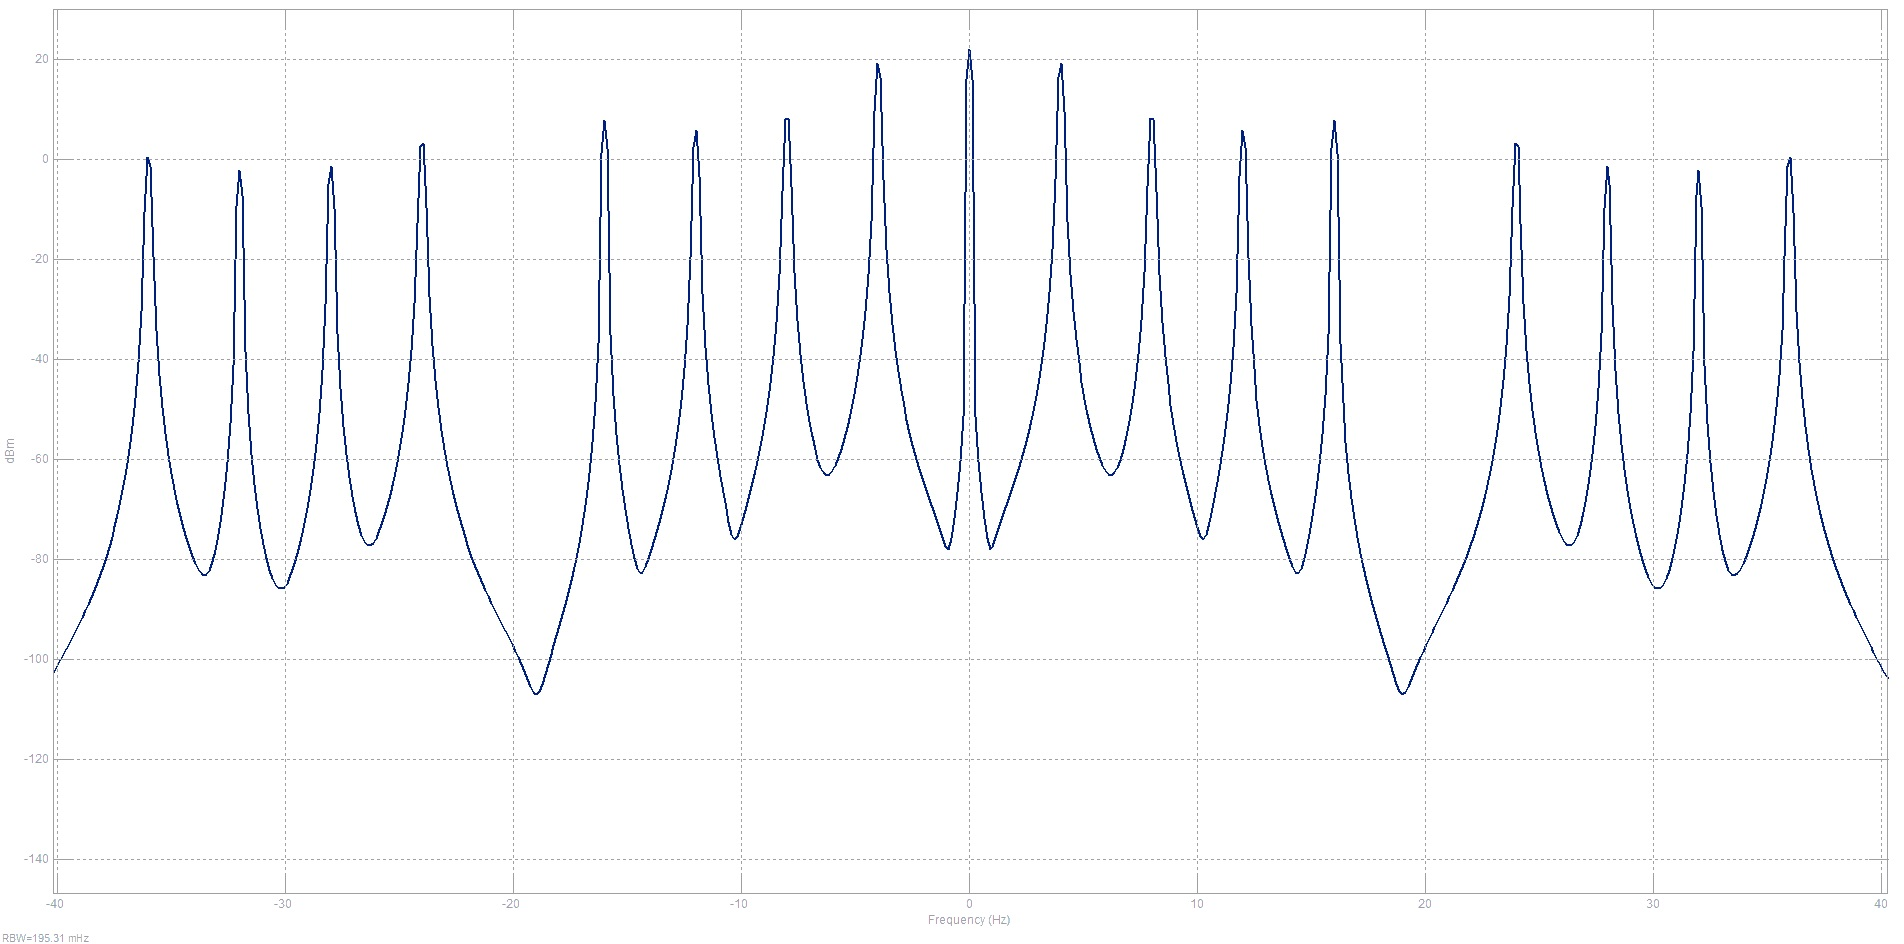
\includegraphics[width=150mm, scale = 0.9]{5_11.jpg}\newline
рис. 15. Спектр прямоугольного сигнала\newline
\end{center}
\end{figure}
\begin{figure}
\begin{center}
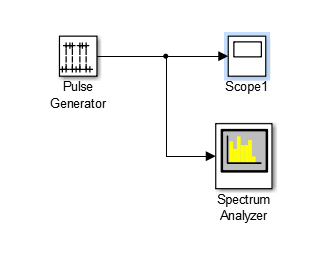
\includegraphics[width=150mm, scale = 0.9]{5_12.jpg}\newline
рис. 16. Модель\newline
\end{center}
\end{figure}
\begin{center}
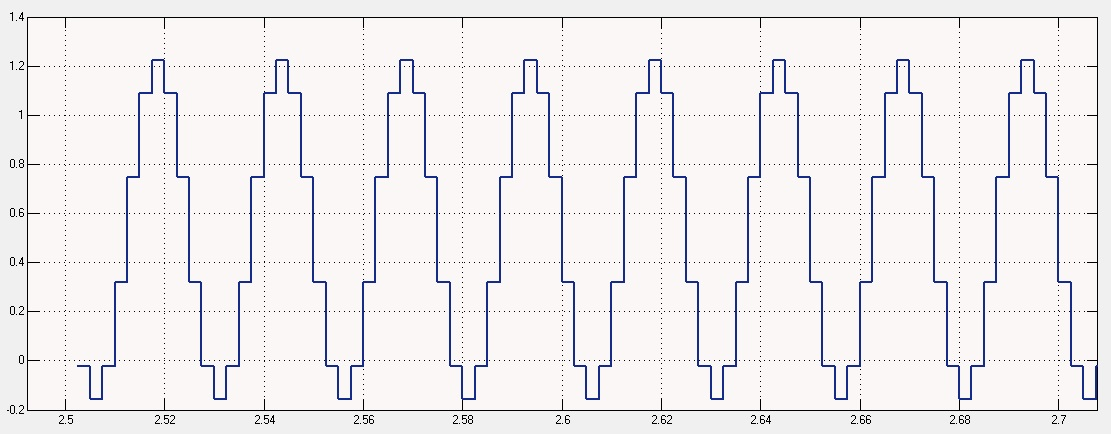
\includegraphics[width=150mm, scale = 0.9]{5_13.jpg}\newline
рис. 17. Треугольный сигнал\newline
\end{center}
\begin{figure}
\begin{center}
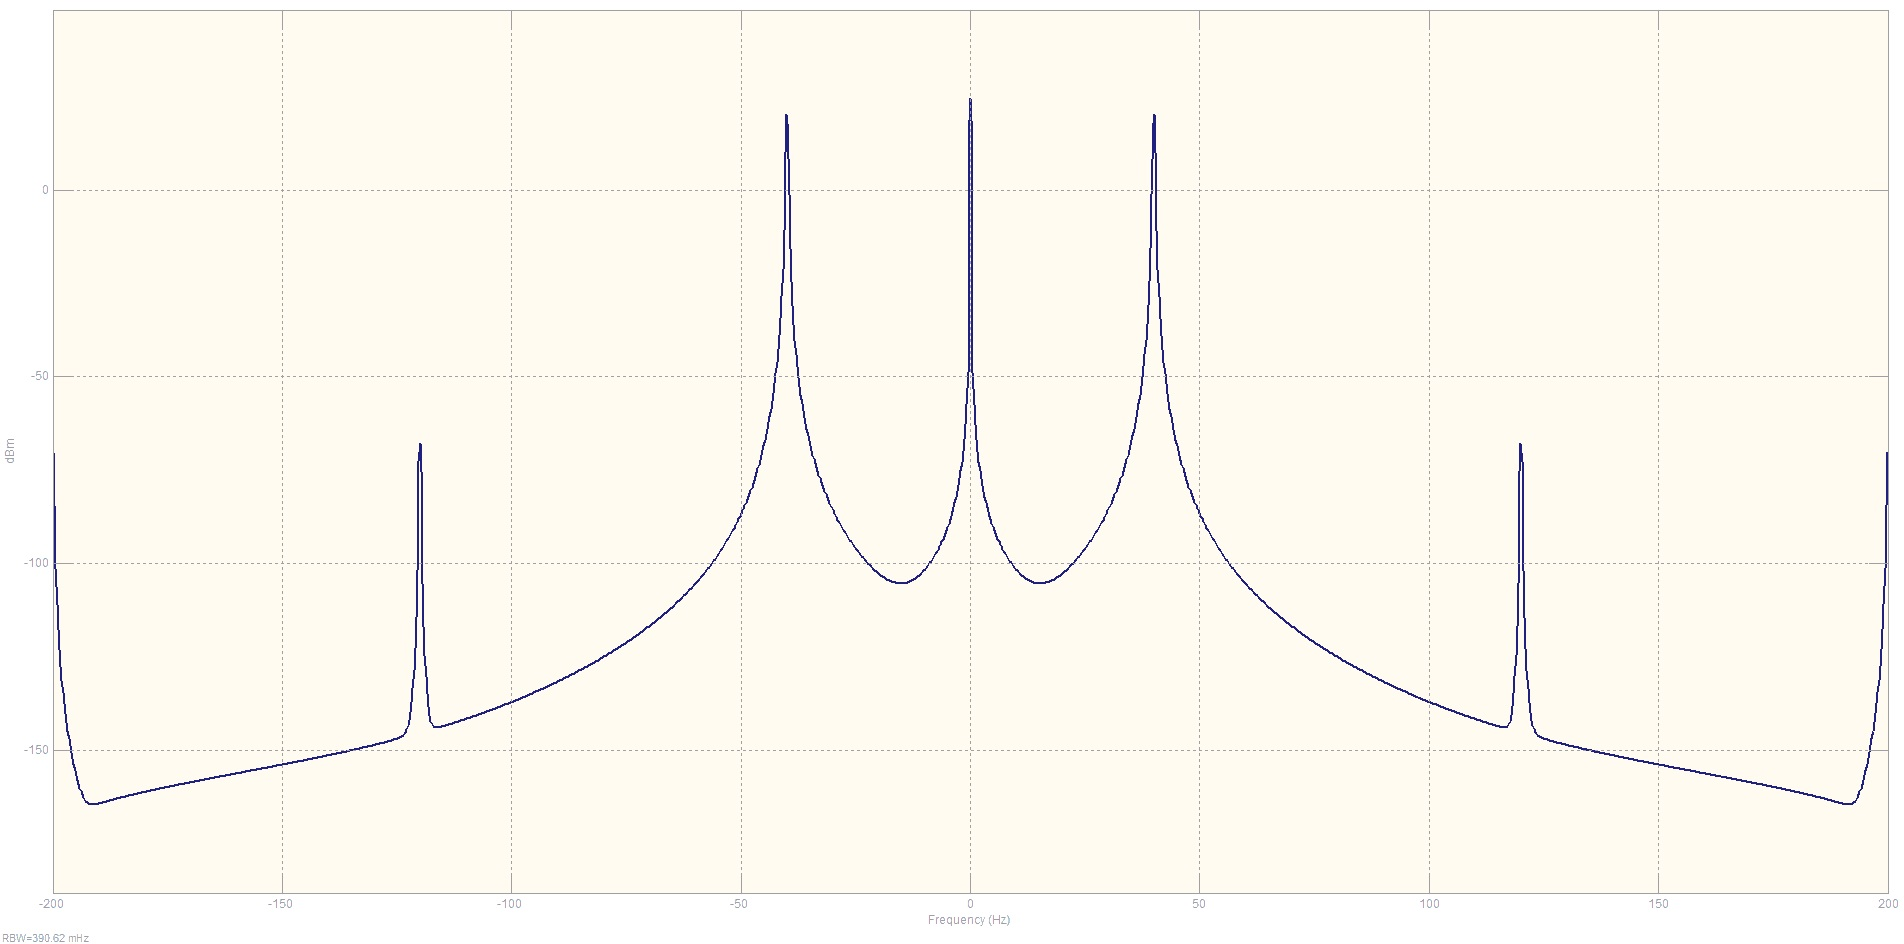
\includegraphics[width=150mm, scale = 0.9]{5_14.jpg}\newline
рис. 18. Спектр треугольного сигнала\newline
\end{center}
\end{figure}
\begin{figure}
\begin{center}
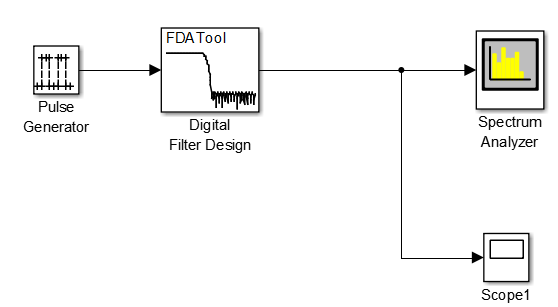
\includegraphics[width=150mm, scale = 0.9]{5_15.jpg}\newline
рис. 19. Модель\newline
\end{center}
\end{figure}
\section{Вывод}
В данной лабораторной работе было проведено моделирование основных видов сигналов: полигармонического, прямоугольного и треугольного, а так же были получены их спектры. Сигналы были полученны как при помощи формул данных функций, так и при помощи среды моделирования Simulink. Спектры сигналов так же были получены обоими вышеприведенными способами. Стоит отметить получение треугольного сигнала, т.к. он был получен не при помощи конкретной формулы, а путем свертки двух прямоугольных сигналов. Это возможно из-за того, что линейная функция может быть полученна как интеграл от двух констант. Таким образом, мы получаем две линейные функции, с отличием в коэфициенте наклона (у одной он положителен, а у другой отрицателен). Так же стоит отметить, что все полученные результаты соответствуют теоретическим ожиданиям.
\chapter{Лабораторная работа №6}
\section{Цель работы}
Изучить воздействие фильтра нижних частот на тестовый сигнал с шумом. Для этого предлагается сгенерировать гармонический сигнал с шумом, затем смоделировать фильтр нижних частот (ФНЧ) и сравнить сигналы до и после фильтрации во временной и частотной областях.
\section{Теоретическая часть}
Фильтр низких частот - один из видов фильтров, эффективно пропускающий частотный спектр сигнала ниже определенной частоты (частоты среза) и уменьшающий частоты сигнала выше этой частоты. Для реализации фильтра в данной лабораторной работе был реализован фильтр Баттерворта. Фильтр Баттерворта проектируется так, чтобы его амплитудно-частотная характеристика была максимально гладкой на частотах полосы пропускания. Порядок фильтра прямопропорционален скорости подавления сигнала выше полосы пропускания. Так же замено, что при более высоком порядке фильтра, частота среза выражена ярче. Амплитудно-частотная характеристика G(w) фильтра Баттерворта n го порядка может быть получена из передаточной функции H(s):
\begin{displaymath}
	G^2(w) = |H^2(s)| = \frac{G_0^2}{1+(\frac{w}{w_c})^2}
\end{displaymath}
где:
\begin{itemize}
\item n — порядок фильтра
\item w_c — частота среза (частота на которой амплитуда равна −3dB)
\item G_0 — коэффициент усиления по постоянной составляющей (усиление на нулевой частоте)
\end{itemize}
Легко заметить, что для бесконечных значений n АЧХ становится прямоугольной функцией, и частоты ниже частоты среза будут пропускаться с коэффициентом усиления G_0, а частоты выше частоты среза будут полностью подавляться. Для конечных значений n спад характеристики будет пологим.
\section{Код matlab}
\begin{verbatim}
x = 0:0.01:4*pi;\newline
f=100*(0:255)/512;\newline
figure\newline
noise=rand(size(x));\newline
y = sin(2*pi*x);\newline
y_noisy = y + 0.3*noise;\newline
plot(x(1:200),y(1:200))\newline
grid\newline
figure\newline
plot(x(1:200),y_noisy(1:200))\newline
grid\newline
[B,A] = butter(16,0.99); синтез ФНЧ Баттерворта\newline 
B=B./sum(B);\newline
A=A./sum(A);\newline
обработка сигнала ФНЧ\newline
figure\newline
y_filtered = conv(y_noisy,[B,A]);\newline
plot(x(1:200),y_filtered(1:200))\newline
grid\newline
выделение спектра\newline
figure\newline
normal_spectrum = fft(y,512);\newline
norm_spectrum = normal_spectrum.*conj(normal_spectrum)/512;\newline
plot(f,norm_spectrum(1:256))\newline
axis([0 max(f) 0 2])\newline
grid\newline
figure\newline
noisy_spectrum = fft(y_noisy,512);\newline
norm_noisy_spectrum = noisy_spectrum.*conj(noisy_spectrum)/512;\newline
plot(f,norm_noisy_spectrum(1:256))\newline
axis([0 max(f) 0 2])\newline
grid\newline
figure\newline
spectrum = fft(y_filtered,512);\newline
norm_filtered_spectrum=spectrum.*conj(spectrum)/512;\newline
plot(f,norm_filtered_spectrum(1:256))\newline
axis([0 max(f) 0 2])\newline
grid\newline
\end{verbatim}
\section{Результаты работы}
\begin{figure}
\begin{center}
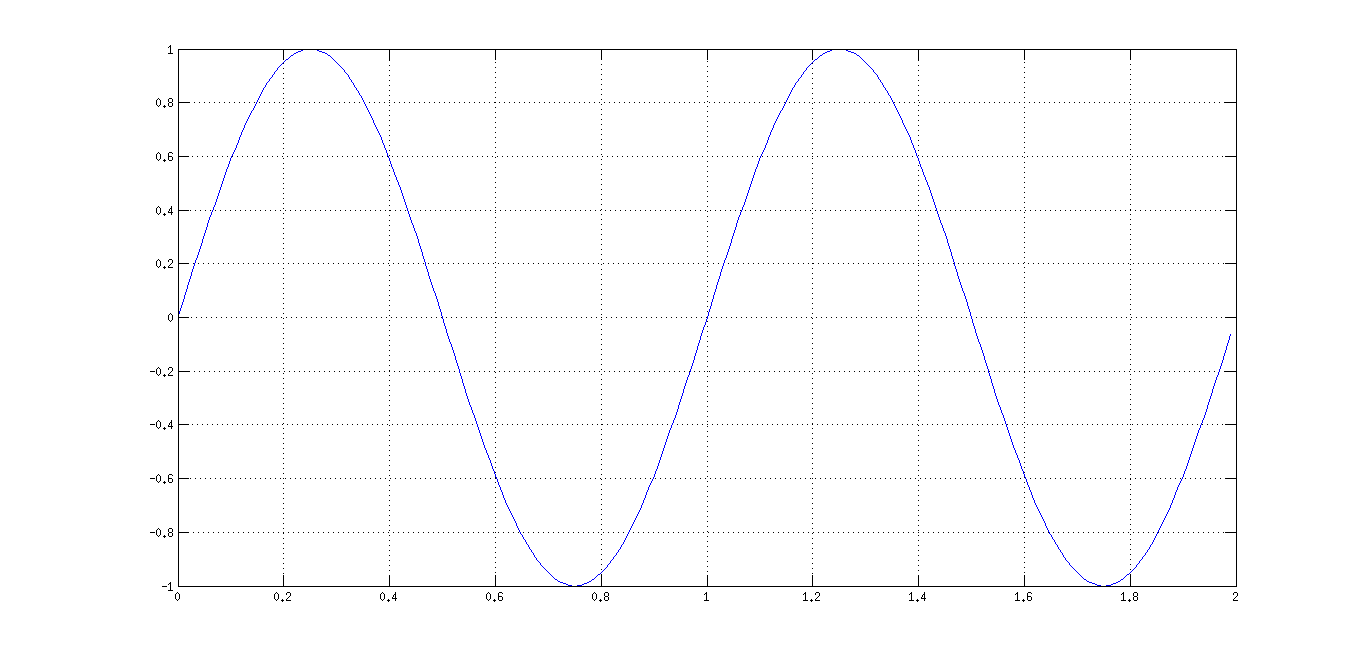
\includegraphics[width=150mm, scale = 0.9]{6_1.png}\newline
рис. 20. Полигармонический сигнал\newline
\end{center}
\end{figure}
\begin{figure}
\begin{center}
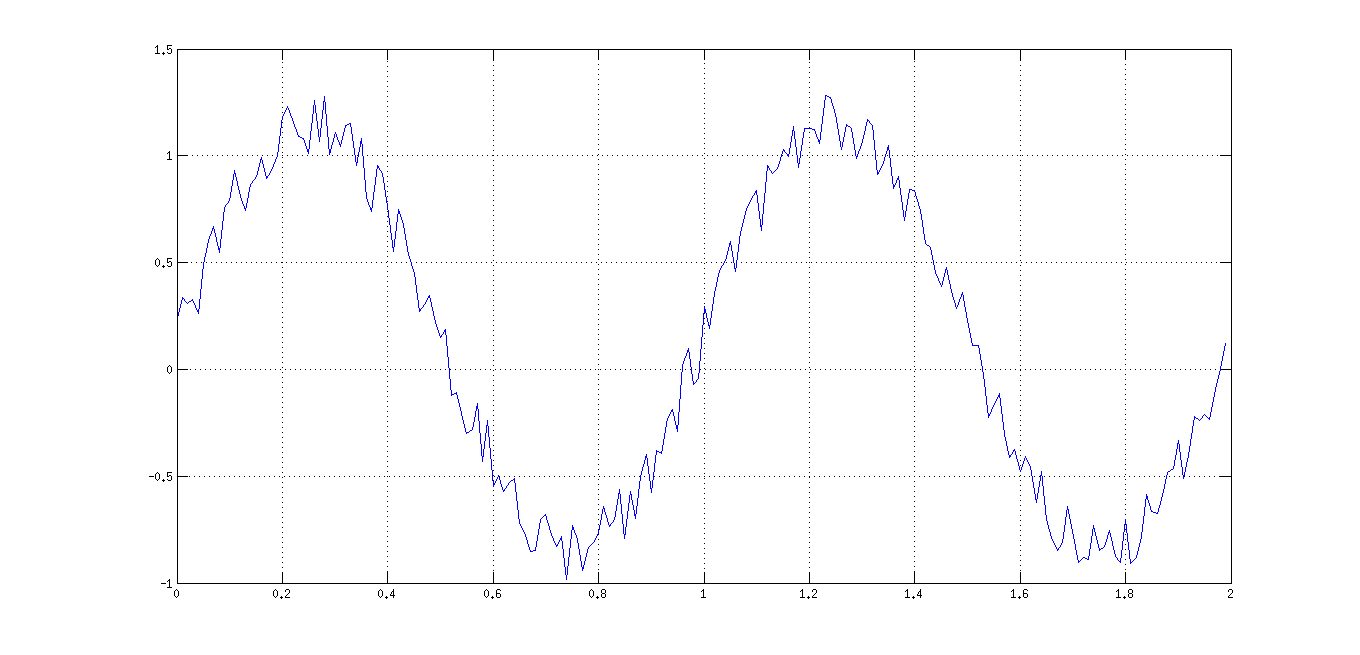
\includegraphics[width=150mm, scale = 0.9]{6_2.png}\newline
рис. 21. Зашумленный полигармонический сигнал\newline
\end{center}
\end{figure}
\begin{figure}
\begin{center}
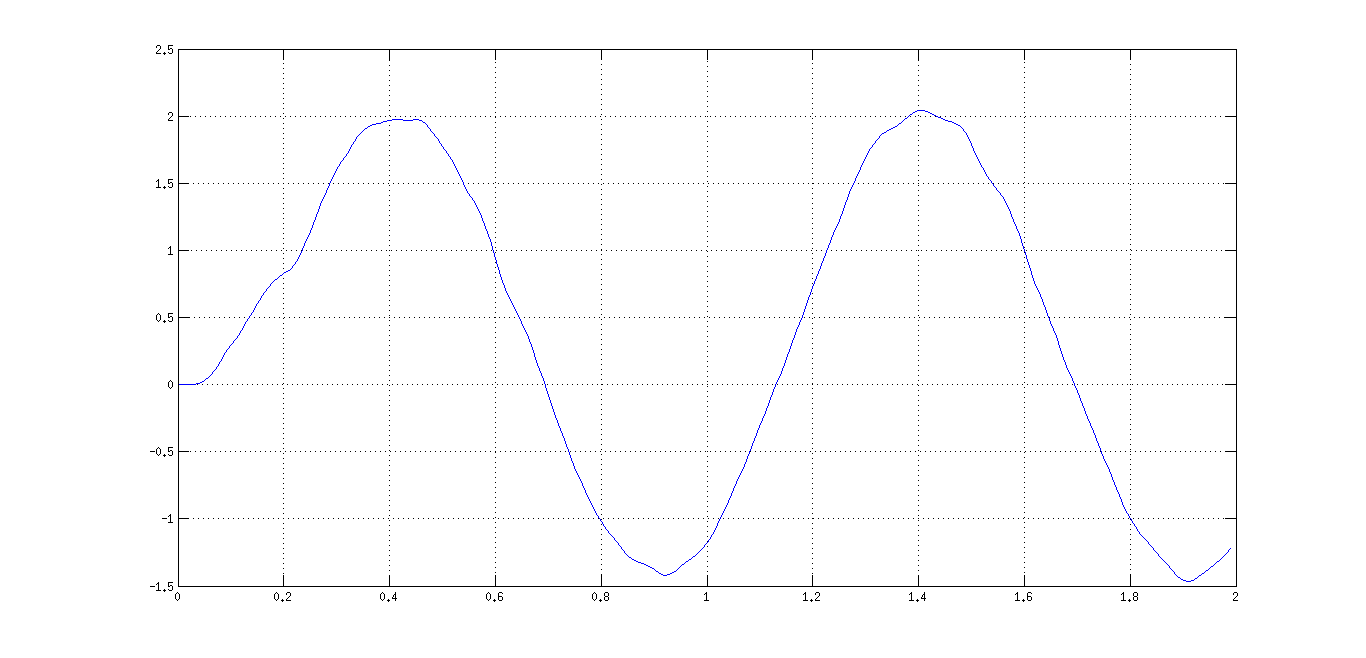
\includegraphics[width=150mm, scale = 0.9]{6_3.png}\newline
рис. 22. Сигнал после фильтрации\newline
\end{center}
\end{figure}
\begin{figure}
\begin{center}
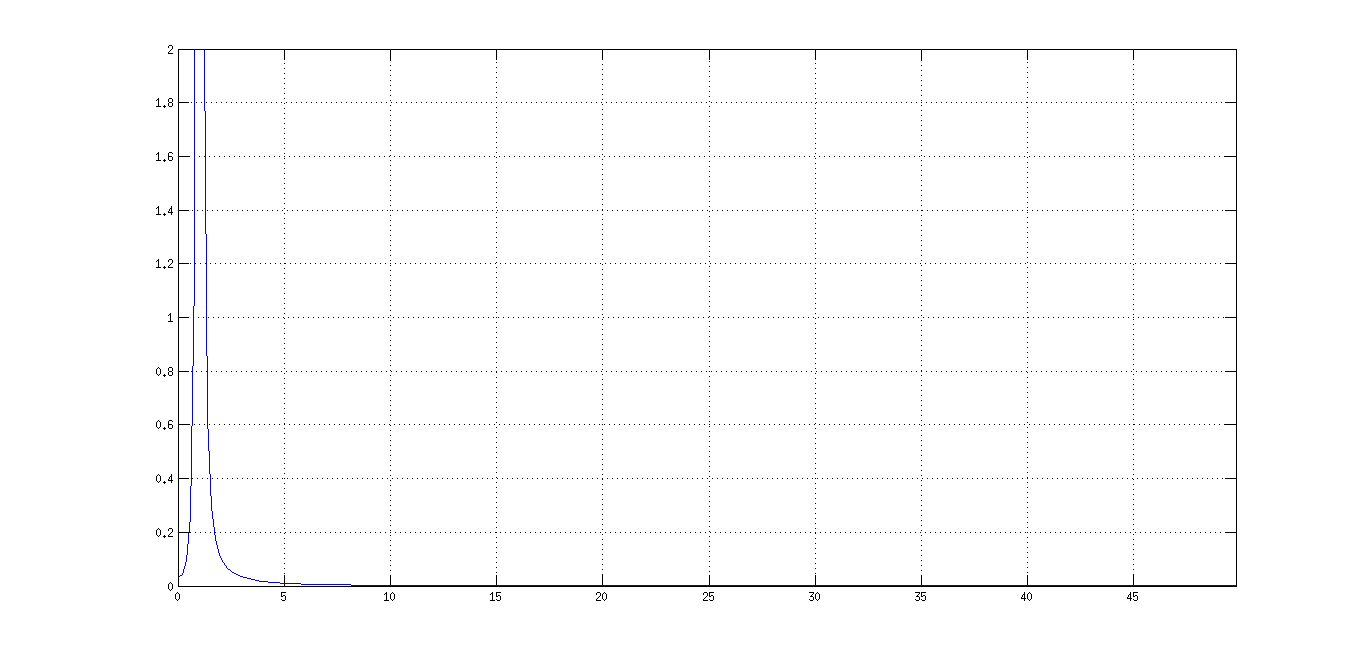
\includegraphics[width=150mm, scale = 0.9]{6_4.png}\newline
рис. 23. Спектр полигармонического сигнала\newline
\end{center}
\end{figure}
\begin{figure}
\begin{center}
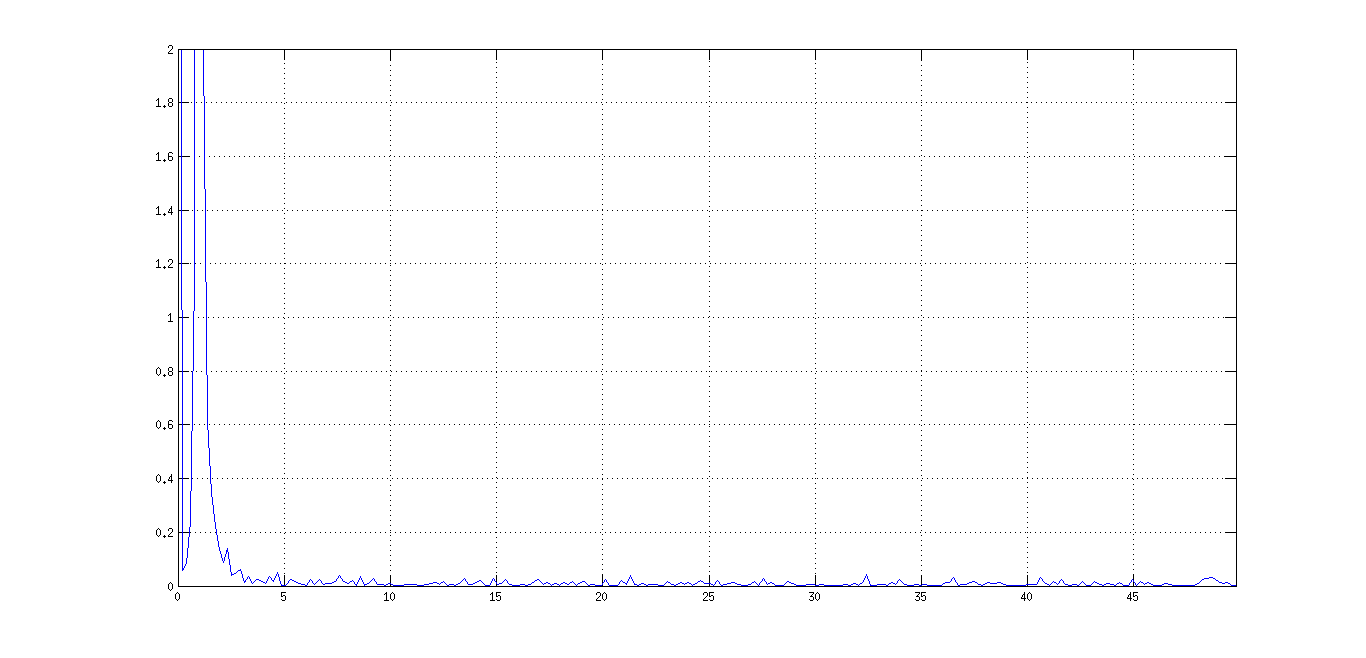
\includegraphics[width=150mm, scale = 0.9]{6_5.png}\newline
рис. 24. Спектр зашумленного сигнала\newline
\end{center}
\end{figure}
\begin{figure}
\begin{center}
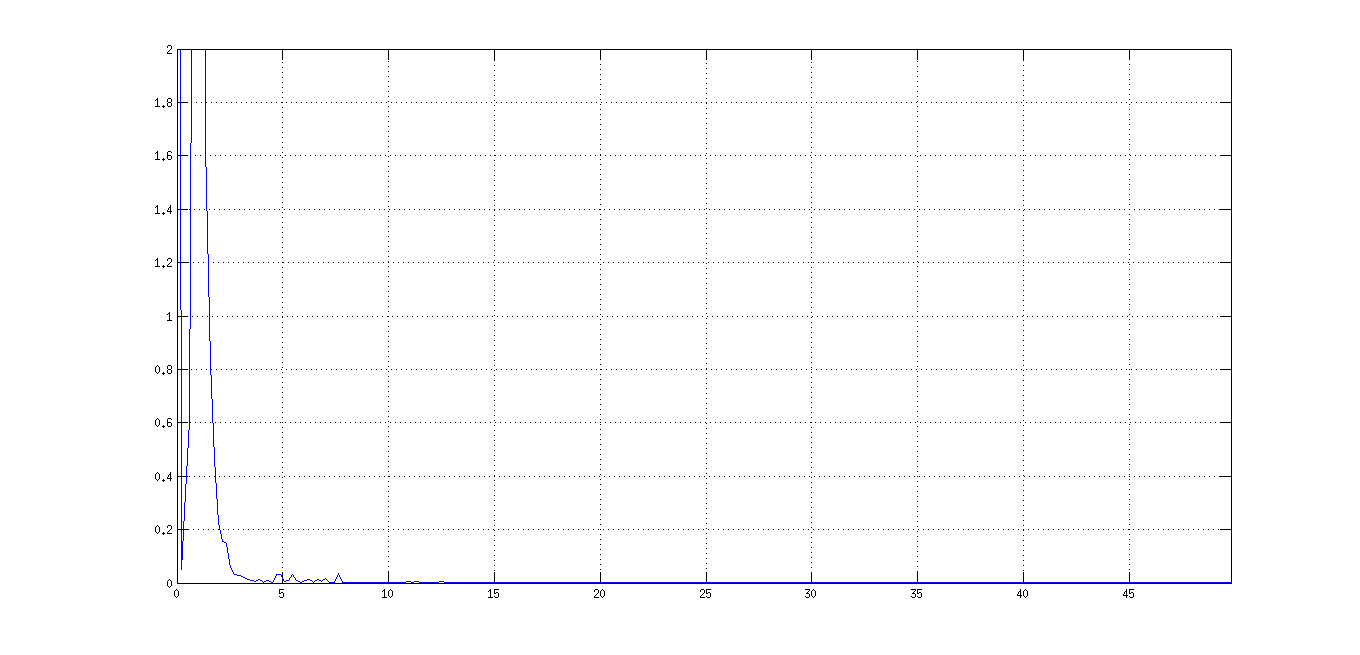
\includegraphics[width=150mm, scale = 0.9]{6_6.png}\newline
рис. 25. Спектр сигнала, прошедшего фильтрацию сигнала\newline
\end{center}
\end{figure}
результаты работы в Simulink
begin{figure}
\begin{center}
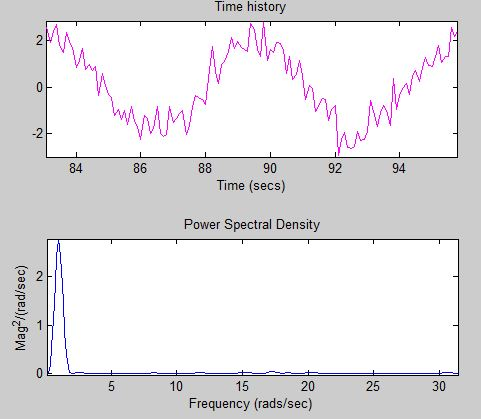
\includegraphics[width=150mm, scale = 0.9]{6_7.jpg}\newline
рис. 26. Спектр зашумленного сигнала\newline
\end{center}
\end{figure}
\begin{figure}
\begin{center}
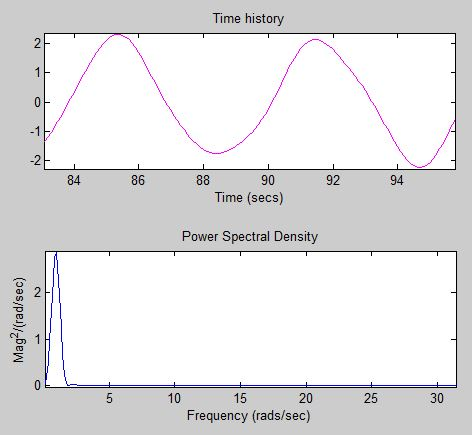
\includegraphics[width=150mm, scale = 0.9]{6_8.jpg}\newline
рис. 27. Спектр отфильтрованного сигнала\newline
\end{center}
\end{figure}
\begin{figure}
\begin{center}
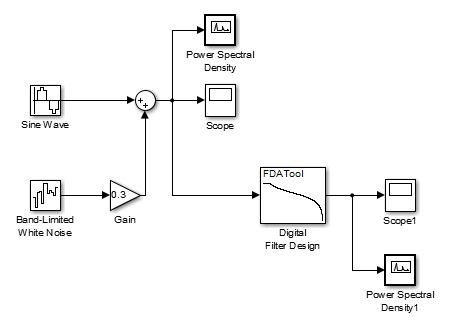
\includegraphics[width=150mm, scale = 0.9]{6_9.jpg}\newline
рис. 28. Модель\newline
\end{center}
\end{figure}
\section{Вывод}
Временная характеристика сигнала после фильтрации фильтром Баттерворта 16 порядка, практически совпадает с исходным сигналом. Незначительные отличия объясняются во-первых, погрешностью вычислений, а во-вторых - погрешностью алгоритма. Для получения идеального сигнала, порядок фильтра должен стремиться к бесконечности, что нереализуемо на практике. Частотная характеристика у исходного, отфильтрованного и зашумленного сигнала очень схожи, однако стоит отметить, что характеристика отфильтрованного сигнала более плавная и ближе к частотной характеристике исходного сигнала, чем частотная характеристика зашумленного сигнала.
\chapter{Лабораторная работа №7}
\section{Постановка задачи}
	\begin{enumerate}
		\item Сгенерировать однотоальный сигнал низкой частоты.
		\item Выполнить амплитудную модуляцию сигнала по закону
				\begin{equation}
					u(t) = (1+MU_m cos(\Omega t))cos(\omega_0 t+\phi_0).
				\end{equation}
		\item Получить спектр модулированного сигнала.
		\item Выполнить модуляцию с подавлением несущей 
				\begin{equation}
					u(t) = MU_m cos(\omega t)cos(\omega_0 t+\phi_0).
				\end{equation}
		      Получить спектр. 
		\item Выполнить однополосную модуляцию:
				\begin{equation}
					u(t) = U_m cos(\omega t)cos(\omega_0 t+\phi_0)+\frac{U_m}{2}\sum_{n=1}^N M_n (cos(\omega_0 + \Omega_n )t + \phi_0 + \Phi_n ),
				\end{equation}
				положив n = 1.
		\item Выполить синхронное детектирование и получить исходный однополосный сигнал.
		\item Рассчитать КПД модуляции
				\begin{equation}
					\eta_A M = \frac{U_m ^2 M^2 /4}{P_U} = \frac{M^2}{M^2 + 2}.
				\end{equation}
	\end{enumerate}
\section{Теоретическая часть}
Амплитудная модуляция - модуляция, при которой сигнал представляет собой произведение информационной огибающей u(t) и гармонического колебания ее заполнения с более высокими частотами. Простейшая форма модулированного сигнала создается при однотональной амплитудной модуляции, при которой несущий сигнал модулируется гармоническим колебанием с одной частотой $\Omega$:
	\begin{equation}
		u(t) = (1+MU_m cos(\Omega t))cos(\omega_0 t+\phi_0).
	\end{equation}
При модуляции с подавлением несущей частоты производится перемножение двух сигналов - модулирующего и несущего, при котором проиходит подавление неcущего колебания. КПД модуляции равен 100\%. 
Физическая сущность подавления несущей заключается в том, что при переходе огибающей биений U(t) через 0 фаза несущей частоты высокочастотного заполнения изменяется на $180^0$.
Синхронное детектирование является одним из способов демодуляции АМ-сигнала. Его суть состоит в умножении частоты сигнала на опорное колебание с несущей частотой. Результат умножения содержит два слагаемых: искомая амплитуда и АМ-сигнал с несущей частотой $2\omega_0$. Эта частота может быть убрана, если пропустить данный сигнал, через ФНЧ.
\section{Код matlab}
\begin{verbatim}
x = 0:0.01:8*pi;\newline
f0 = 0.1;\newline
\newline
y = sin(2*pi*f0*x);\newline
figure\newline
plot(x(1:1000),y(1:1000), 'LineWidth', 2)\newline
grid\newline
\newline
spectrum = fft(y, 512);\newline
norm_spectrum = spectrum.*conj(spectrum)/512;\newline
f = 100*(0:255)/512;\newline
figure\newline
plot(f, norm_spectrum(1:256), 'LineWidth', 2)\newline
axis([0 max(f) 0 70])\newline
grid\newline
\newline
Fc = 10*f0;\newline
Fs = 100*f0;\newline
U = ammod(y, Fc, Fs, 0, 1);\newline
figure \newline
plot(x(1:1000), U(1:1000),  'LineWidth', 2)\newline
grid\newline
\newline
 u_spectrum = fft(U, 512);\newline
 norm_u_spectrum = u_spectrum.*conj(u_spectrum)/512;\newline
 figure\newline
 plot(f, norm_u_spectrum(1:256))\newline
 axis([0 max(f) 0 70])\newline
 grid\newline
\newline
Fc = 10*f0;\newline
Fs = 100*f0;\newline
U = ammod(y, Fc, Fs);\newline
figure \newline
plot(x(1:1000), U(1:1000), 'LineWidth', 2)\newline
grid\newline
\newline
u_spectrum = fft(U, 512);\newline
norm_u_spectrum = u_spectrum.*conj(u_spectrum)/512;\newline
figure\newline
plot(f, norm_u_spectrum(1:256))\newline
axis([0 max(f) 0 70])\newline
grid\newline
\newline
Fc = 10*f0;\newline
Fs = 100*f0;\newline
U = ssbmod(y, Fc, Fs, [], 'upper');\newline
figure \newline
plot(x(1:500), U(1:500), 'LineWidth', 2)\newline
grid\newline
\newline
u_spectrum = fft(U, 512);\newline
norm_u_spectrum = u_spectrum.*conj(u_spectrum)/512;\newline
figure\newline
plot(f, norm_u_spectrum(1:256))\newline
axis([0 max(f) 0 70])\newline
grid\newline
\newline
[b, a] = butter(10, Fc*2/Fs);\newline
z = ssbdemod(U, Fc, Fs, 0, b, a);\newline
figure\newline
plot(x(1:1000), z(1:1000), 'LineWidth', 2)\newline
grid\newline
\newline
du_spectrum = fft(U, 512);\newline
norm_du_spectrum = du_spectrum.*conj(du_spectrum)/512;\newline
figure\newline
plot(f, norm_du_spectrum(1:256))\newline
axis([0 max(f) 0 70])\newline
grid\newline
\newline 
M = 0.5;\newline
n = M^2/(M^2+2)\newline
\end{verbatim} 
\section{Результаты работы}
\begin{figure}
\begin{center}
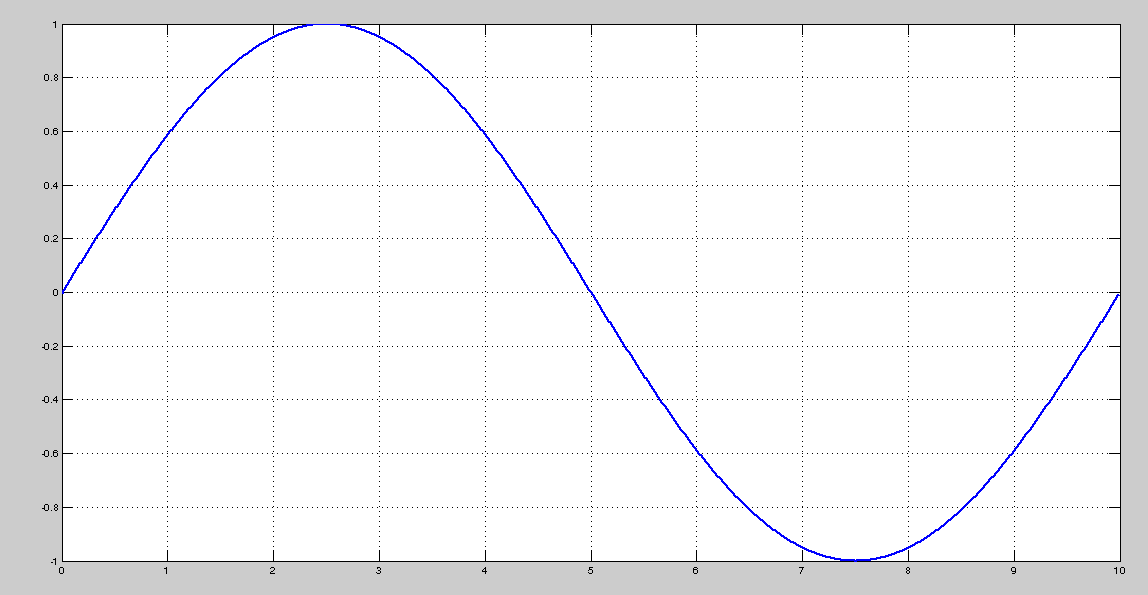
\includegraphics[width=150mm, scale = 0.9]{7_1.png}\newline
рис. 29. Исходный сигнал\newline
\end{center}
\end{figure}
\begin{figure}
\begin{center}
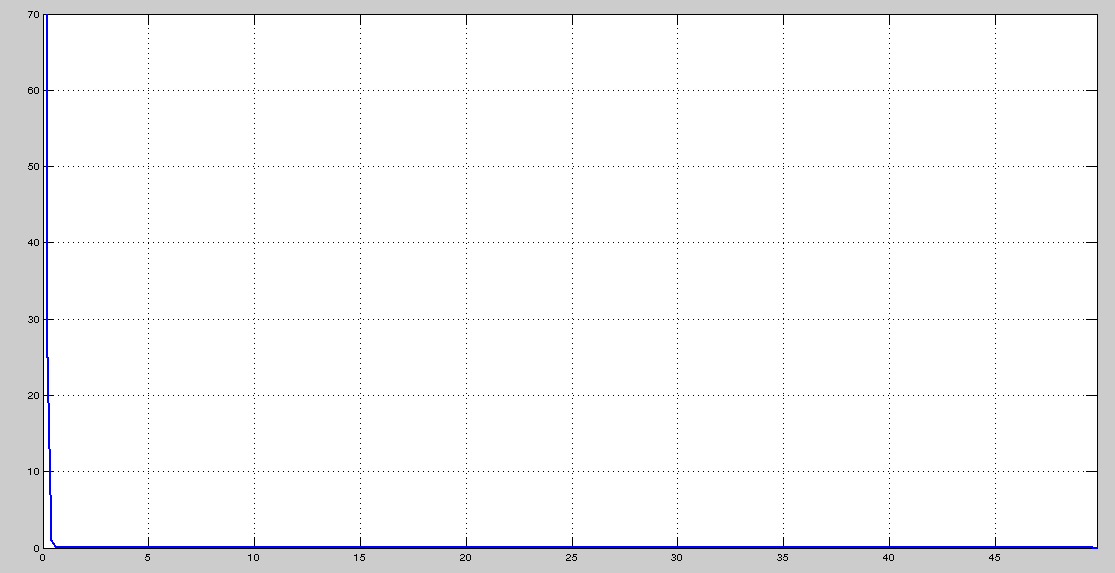
\includegraphics[width=150mm, scale = 0.9]{7_2.png}\newline
рис. 30. Спектр исходного сигнала\newline
\end{center}
\end{figure}
\begin{figure}
\begin{center}
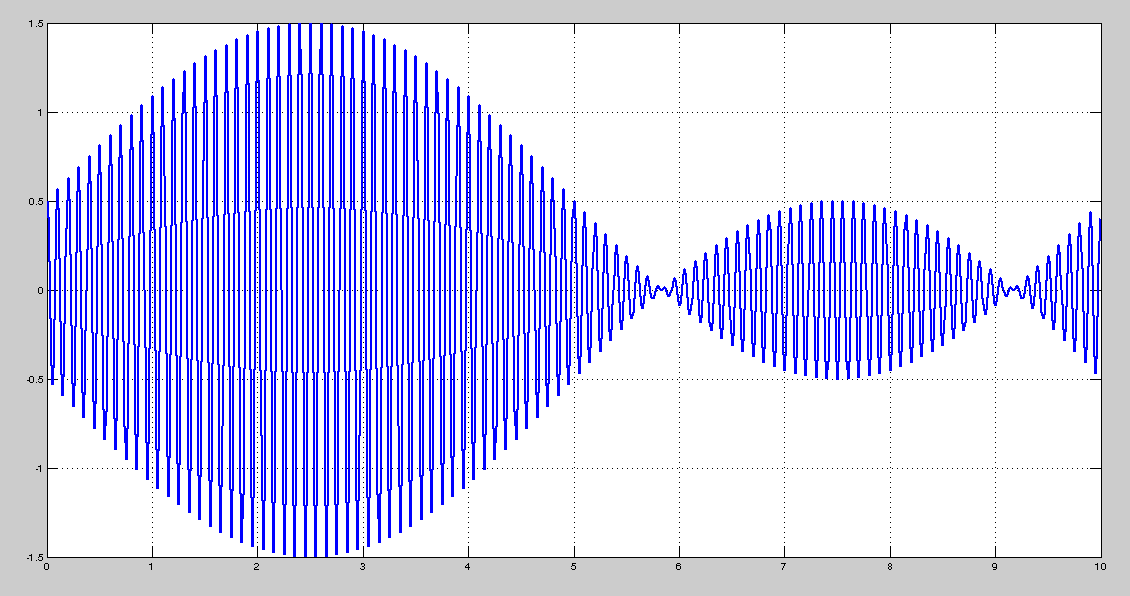
\includegraphics[width=150mm, scale = 0.9]{7_3.png}\newline
рис. 31. Модуляция с М = 0.5\newline
\end{center}
\end{figure}
\begin{figure}
\begin{center}
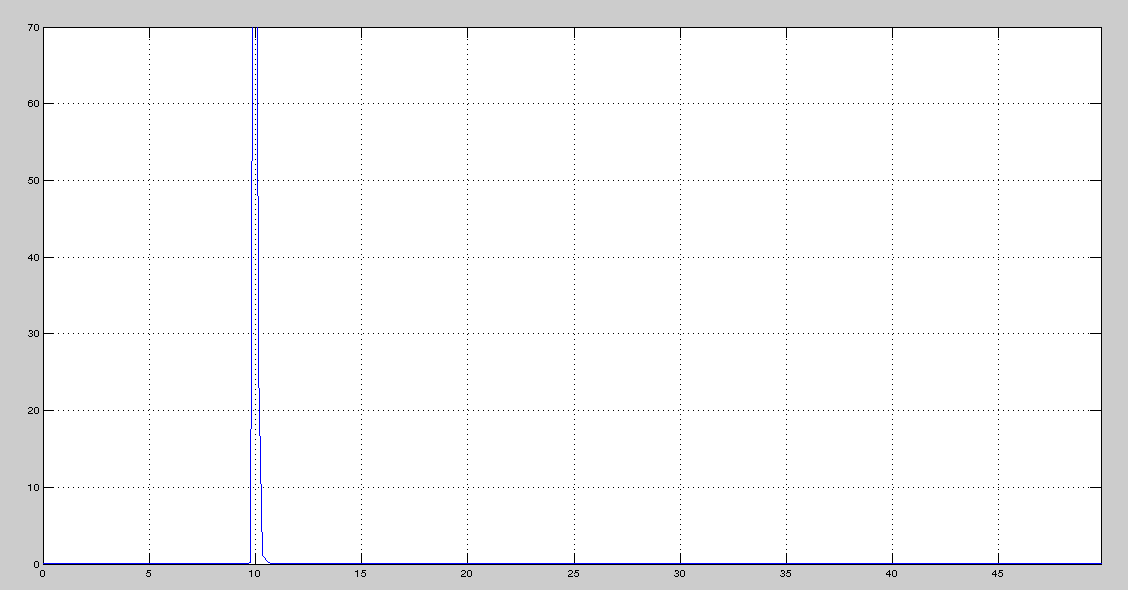
\includegraphics[width=150mm, scale = 0.9]{7_4.png}\newline
рис. 32. Спектр сигнала с М=0.5\newline
\end{center}
\end{figure}
\begin{figure}
\begin{center}
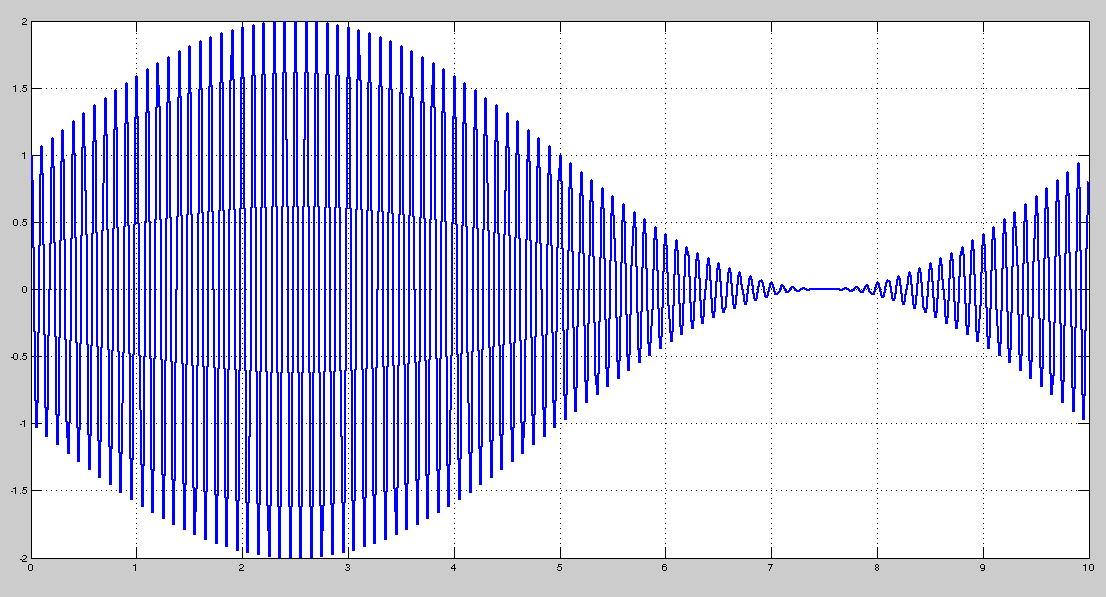
\includegraphics[width=150mm, scale = 0.9]{7_5.png}\newline
рис. 33. Модуляция с М=1\newline
\end{center}
\end{figure}
\begin{figure}
\begin{center}
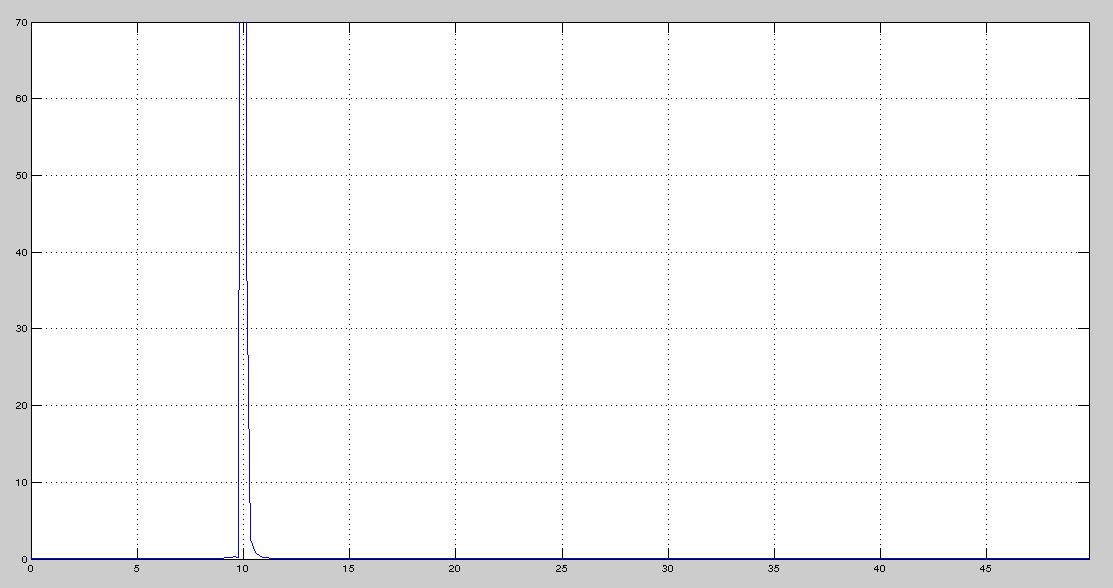
\includegraphics[width=150mm, scale = 0.9]{7_6.png}\newline
рис. 34. Спектр сигнала с М = 1\newline
\end{center}
\end{figure}
begin{figure}
\begin{center}
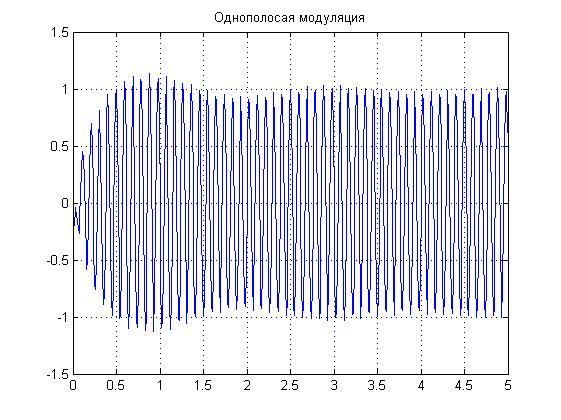
\includegraphics[width=150mm, scale = 0.9]{7_7.jpg}\newline
рис. 35. Сигнал с М = 5\newline
\end{center}
\end{figure}
\begin{figure}
\begin{center}
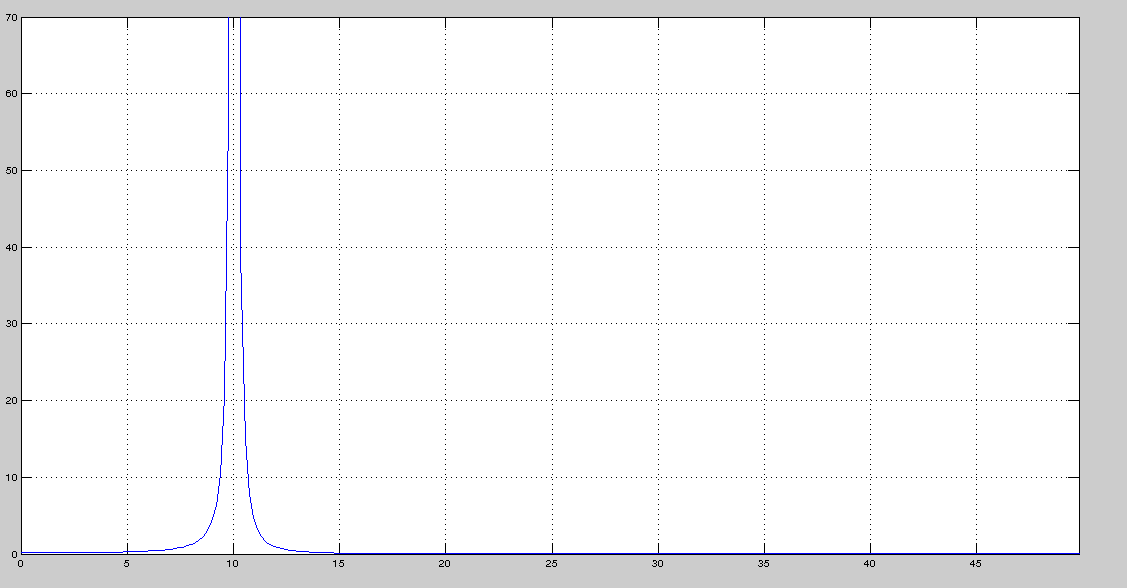
\includegraphics[width=150mm, scale = 0.9]{7_8}\newline
рис. 36. Спектр сигнала с М = 5\newline
\end{center}
\end{figure}
\begin{figure}
\begin{center}
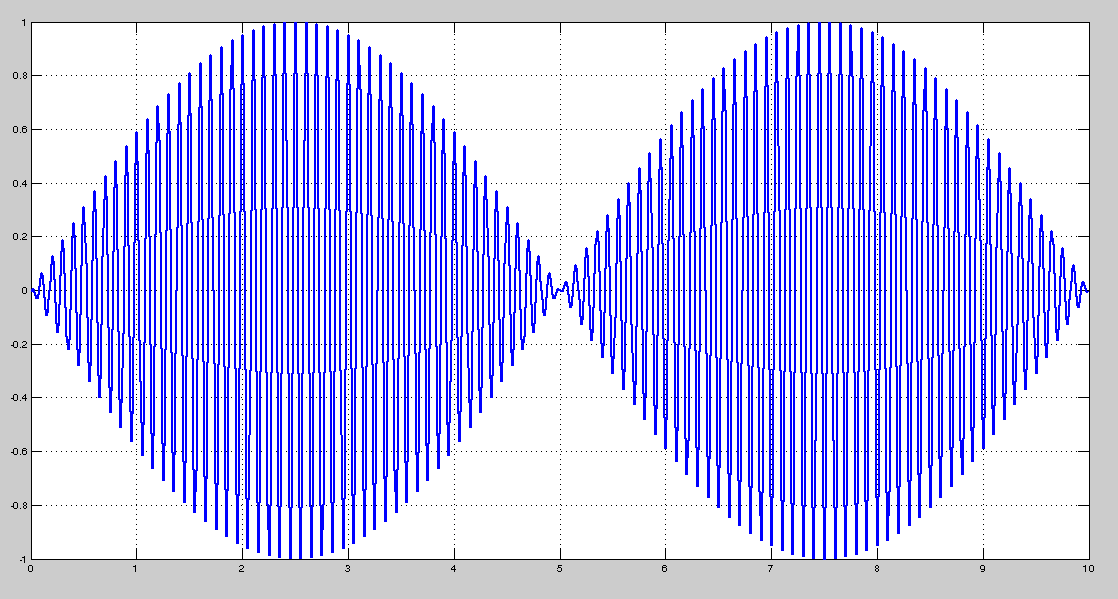
\includegraphics[width=150mm, scale = 0.9]{7_9}\newline
рис. 37. Модуляция с подавлением несущей\newline
\end{center}
\end{figure}
\begin{figure}
\begin{center}
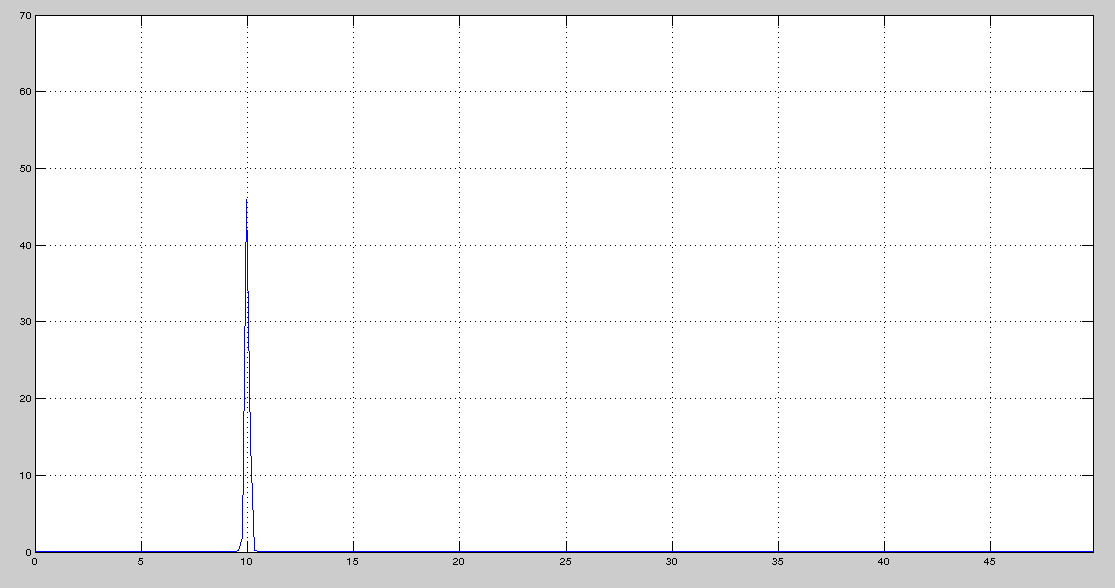
\includegraphics[width=150mm, scale = 0.9]{7_10.png}\newline
рис. 38. Спектр сиганала с подавлением несущей \newline
\end{center}
\end{figure}
\begin{figure}
\begin{center}
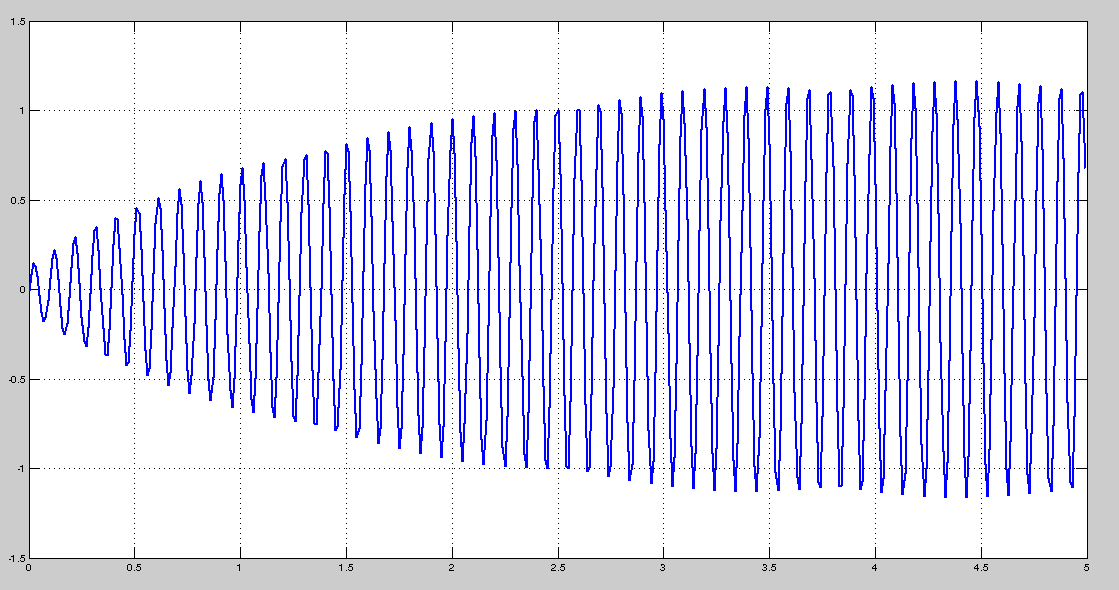
\includegraphics[width=150mm, scale = 0.9]{7_11.png}\newline
рис. 39. Однополосный АМ-сигнал\newline
\end{center}
\end{figure}
\begin{figure}
\begin{center}
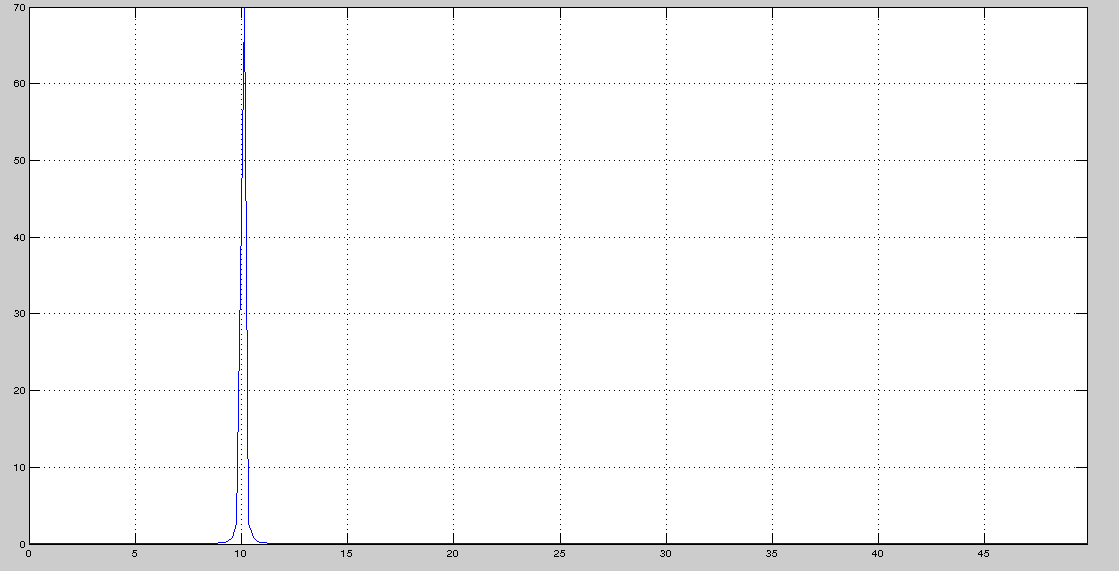
\includegraphics[width=150mm, scale = 0.9]{7_12.png}\newline
рис. 40. Спектр однополосного модулированного сигнала\newline
\end{center}
\end{figure}
\begin{figure}
\begin{center}
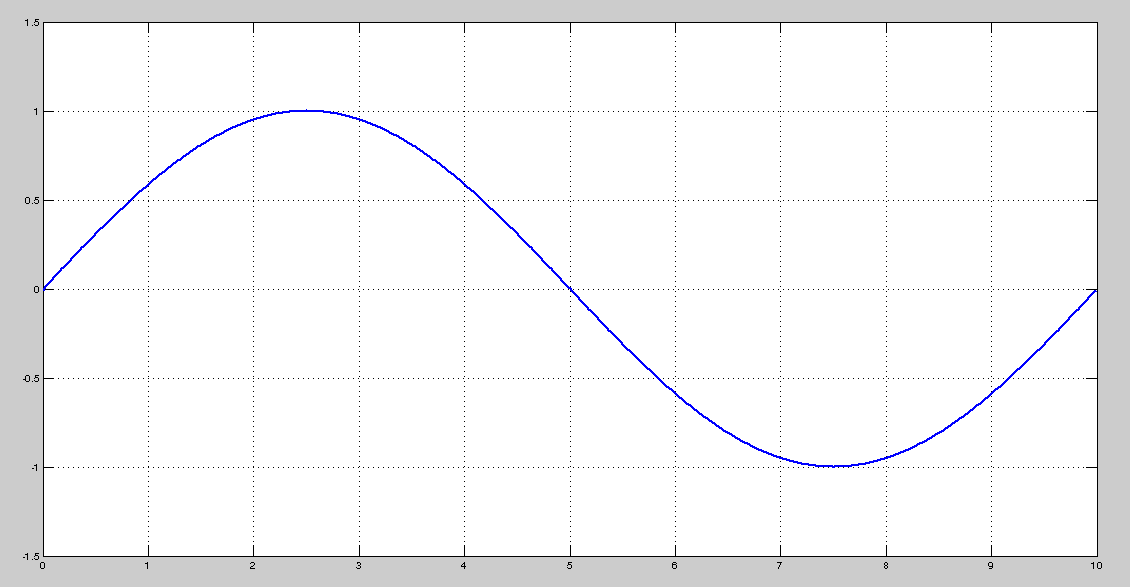
\includegraphics[width=150mm, scale = 0.9]{7_13.png}\newline
рис. 41. Демодулированный сигнал\newline
\end{center}
\end{figure}
\begin{figure}
\begin{center}
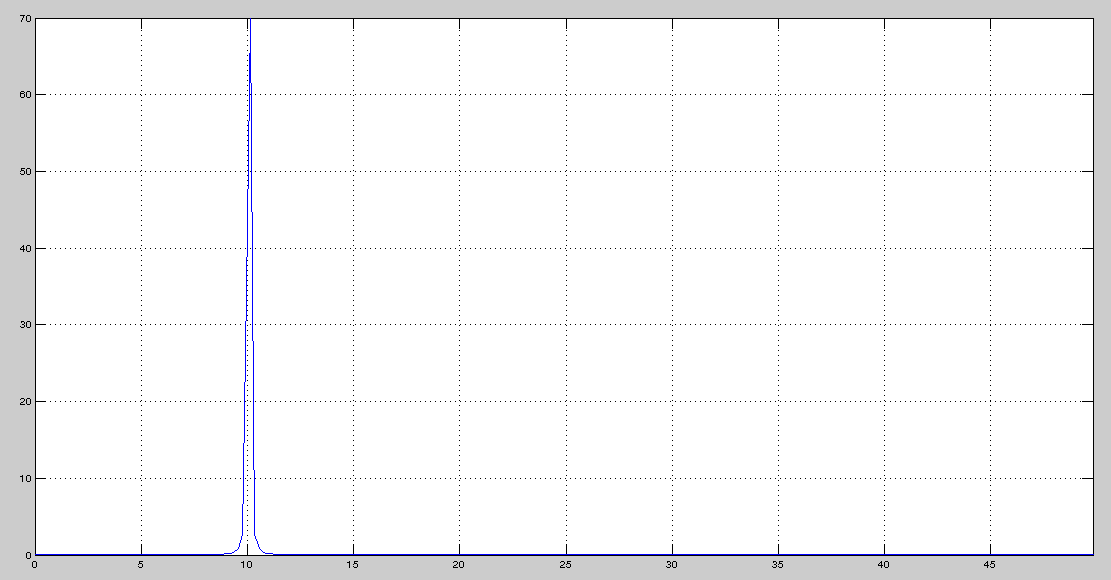
\includegraphics[width=150mm, scale = 0.9]{7_14.png}\newline
рис. 42. Спектр демодулированного сигнала\newline
\end{center}
\end{figure}
Для глубины модулирования 1 КПД равен 0.1111%
Моделирование в среде Simulink
\begin{figure}
\begin{center}
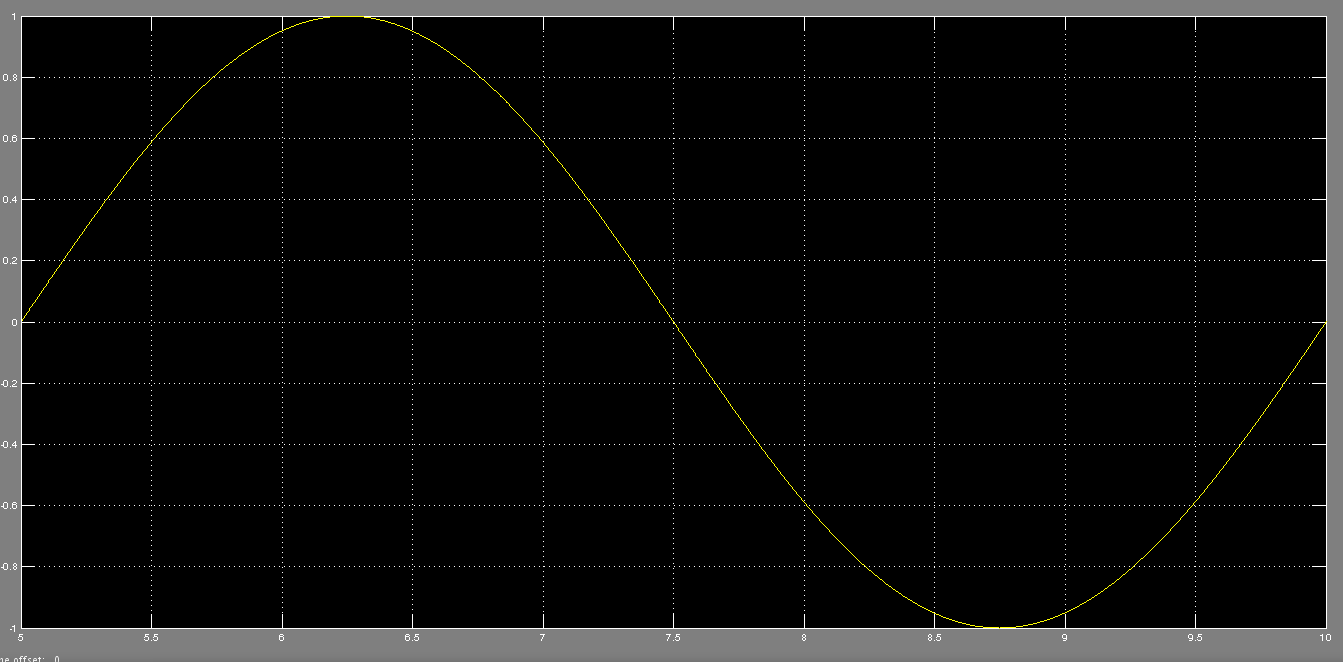
\includegraphics[width=150mm, scale = 0.9]{7_15.png}\newline
рис. 43. Исходный сигнал\newline
\end{center}
\end{figure}
\begin{figure}
\begin{center}
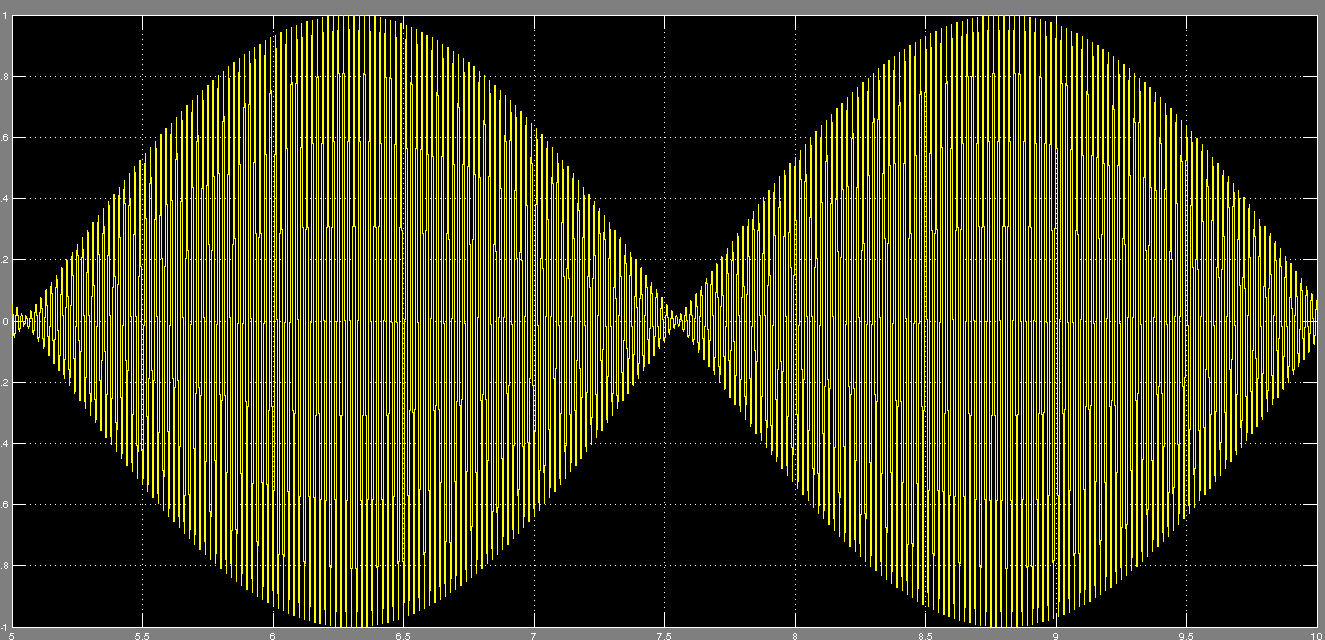
\includegraphics[width=150mm, scale = 0.9]{7_16.png}\newline
рис. 44. Модулированный сигнал\newline
\end{center}
\end{figure}
\begin{figure}
\begin{center}
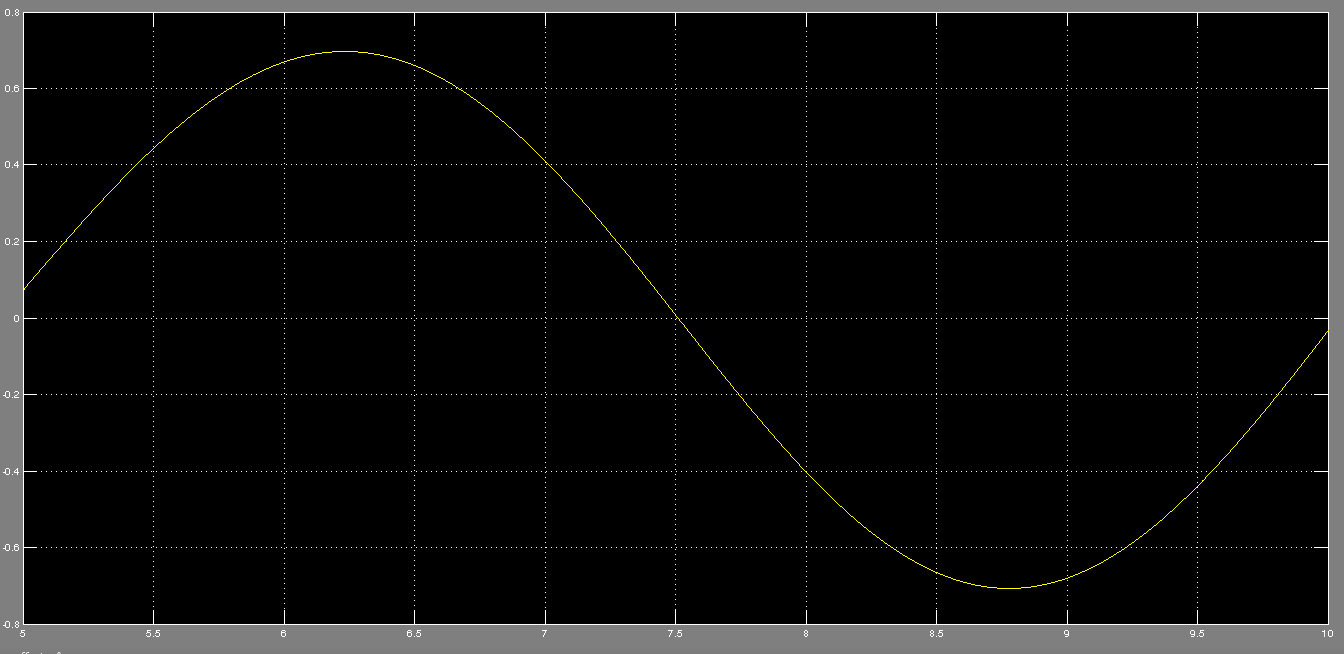
\includegraphics[width=150mm, scale = 0.9]{7_17}\newline
рис. 45. Демодулированный сигнал\newline
\end{center}
\end{figure}
\begin{figure}
\begin{center}
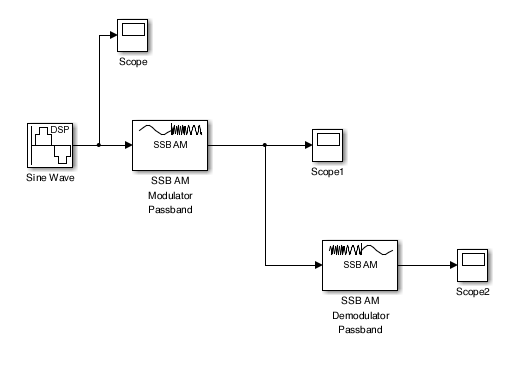
\includegraphics[width=150mm, scale = 0.9]{7_18}\newline
рис. 46. Модель\newline
\end{center}
\end{figure}
\begin{figure}
\begin{center}
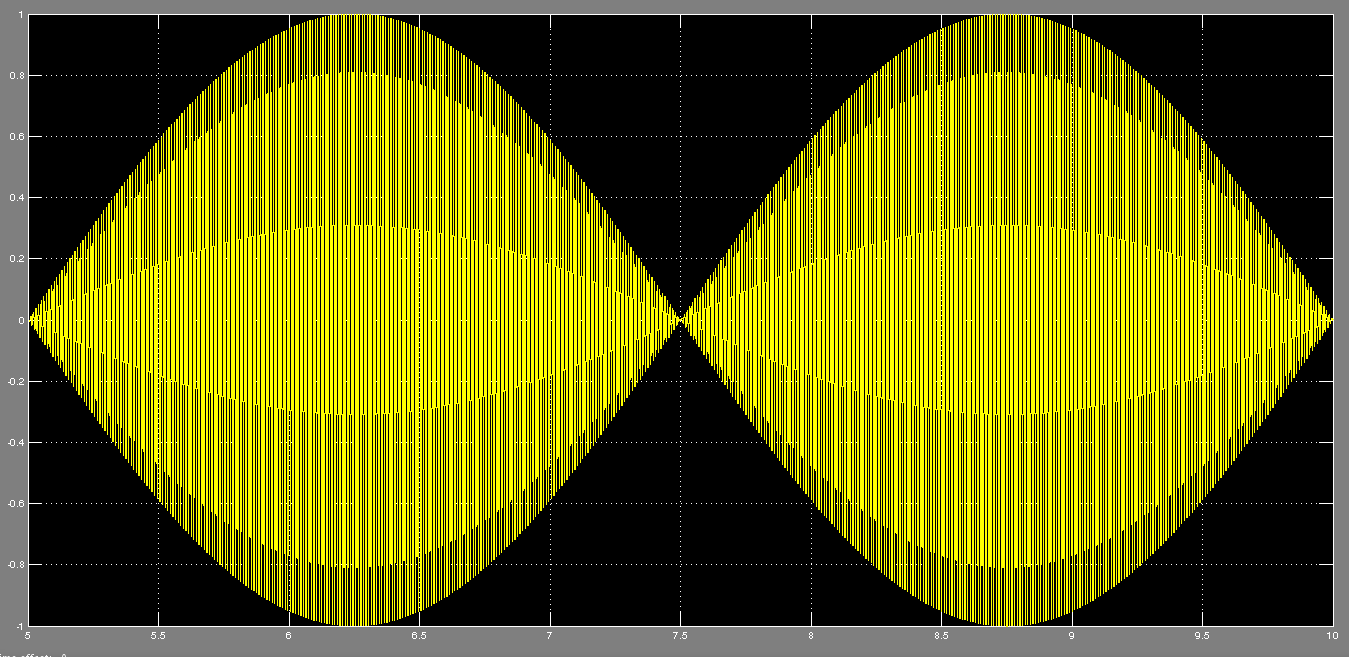
\includegraphics[width=150mm, scale = 0.9]{7_19}\newline
рис. 47. Сигнал БАМ\newline
\end{center}
\end{figure}
\begin{figure}
\begin{center}
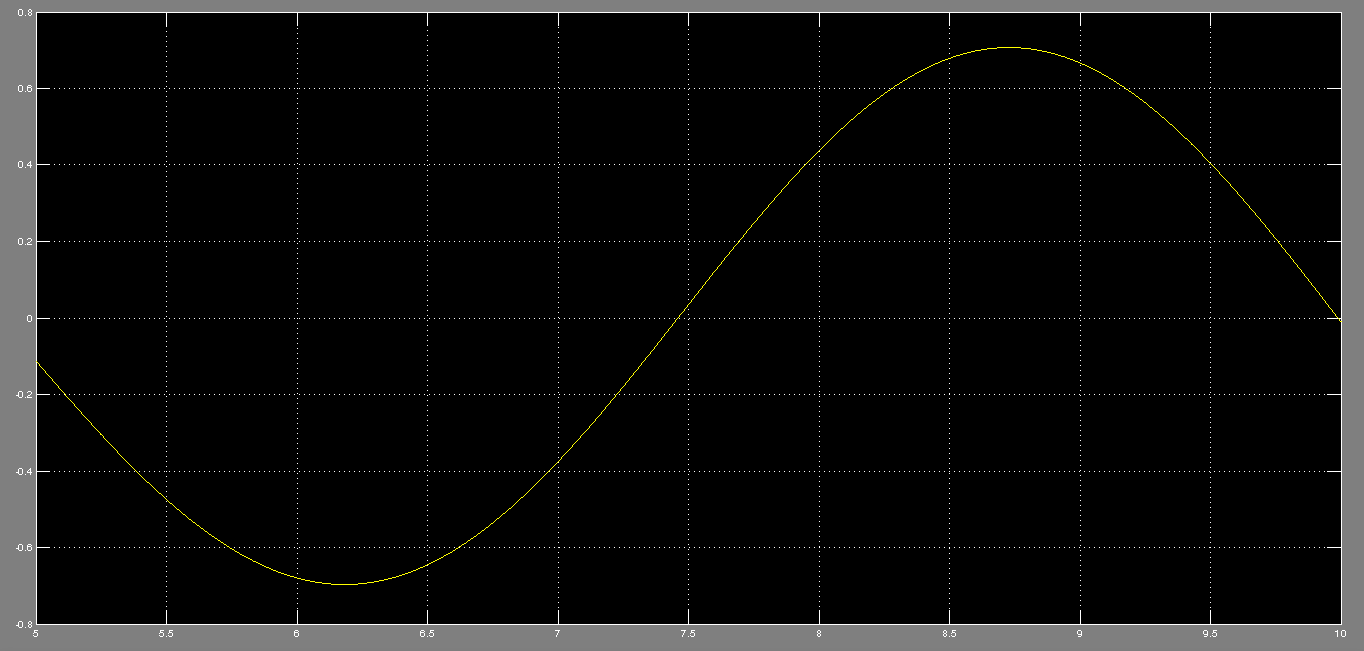
\includegraphics[width=150mm, scale = 0.9]{7_20.png}\newline
рис. 48. Демодулированный БАМ сигнал \newline
\end{center}
\end{figure}
\begin{figure}
\begin{center}
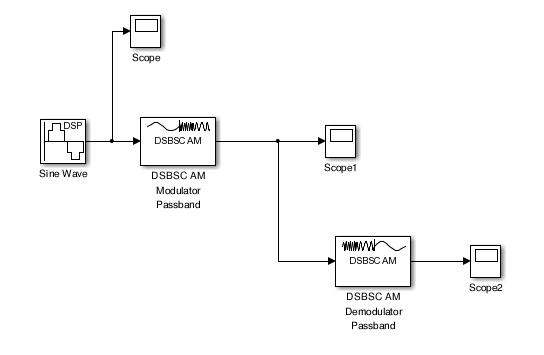
\includegraphics[width=150mm, scale = 0.9]{7_21.png}\newline
рис. 49. Модель\newline
\end{center}
\end{figure}
\section{Вывод}
В данной лабораторной работе был сгенерирован низкочастотный гармонический сигнал и проведена его амплитудная модуляция, баланстная амплитудная модуляция, однополосная амплитудная модуляция, а так же последующая демодуляция. Все результаты соответствуют ожиданиям.
Амплитудная модуляция применяется на низких частотах (не выше коротких волн), что обусловлено низким КПД использования энергии модулированных сигналов.Основным применением амплитудной модуляции является передача сигналов звуковой частоты.
Для получения колебаний боковых частот без несущей применяют так называемую балансную модуляцию, основанную на том, что складывают два АМ колебания, у которых колебания боковых частот находятся в фазе, а несущих - в пративофазе (или берут разность двух АМ колебаний, у которых боковые частоты в противофазе, а несущие - в фазе).КПД такой модуляции становится равно 100 процентам.
Рассмотренная в предыдущем разделе двухполосная АМ с подавленной несущей имеет преимущества перед обычной АМ только в энергетическом плане - за счет устранения несущего колебания. Ширина спектра при этом по-прежнему вдвое больше, чем у модулирующего сигнала. Однако спектры двух боковых полос АМ-сигнала являются зеркальным отражением друг друга, то есть они несут одну и ту же информацию. Поэтому одну из боковых полос можно удалить. Получающаяся модуляция называется однополосной (английский термин - Single Side Band, SSB).
В зависимости от того, какая боковая полоса сохраняется, говорят об однополосной модуляции с использованием верхней или нижней боковой полосы.
Итак, однополосный сигнал можно представить как сумму двух АМ-сигналов, несущие колебания которых имеют одну и ту же частоту, но сдвинуты по фазе друг относительно друга на 90°. Амплитудными функциями этих АМ-сигналов являются модулирующий сигнал и его квадратурное дополнение. В зависимости от того, складываются эти два АМ-сигнала или вычитаются (а точнее, какая из двух несущих опережает другую по фазе), формируется однополосный сигнал с верхней или нижней боковой полосой.
Синхронное детектирование является одним из способов демодуляции АМ-сигнала. Его суть состоит в умножении частоты сигнала на опорное колебание с несущей частотой. Результат умножения содержит два слагаемых: искомая амплитуда и АМ-сигнал с несущей частотой 2ω0 , который легко удаляется путем пропускания сигнала через ФНЧ (например через фильт Баттерворта).
\chapter{Лабораторная работа №8}
\section{Постановка задачи}
\begin{enumerate}
\item 
Сгенерировать однотональный сигнал низкой частоты.
\item
Выполнитьфазовую модуляцию/демодуляцию сигнала по закону $u(t)=(U_m\cos(\omega t=ks(t))$ , используя встроенную функцию MatLab pmmod, pmdemod.
\item
Получить спектр модулированного сигнала.
\item
Выполнить частотную модуляцию/демодуляцию по закону 
\begin{equation}
u(t)=U_m\cos (\omega _0 t+k \int_0^t s(t)dt=\phi _0)
\end{equation}
используя встроенные функции Matlab fmmod, fmdemod.
\end{enumerate}
\section{Теоретическая часть}
Частотная модуляция — вид аналоговой модуляции, при котором информационный сигнал управляет частотой несущего колебания. По сравнению с амплитудной модуляцией здесь амплитуда остаётся постоянной.\newline
Фазовая модуляция — один из видов модуляции колебаний, при которой фаза несущего колебания управляется информационным сигналом. Фазомодулированный сигнал s(t) имеет следующий вид:
\begin{equation} 
s(t) = g(t) \sin[2 \pi f_c t + \varphi(t)] ,
\end{equation}
где $g(t)$ — огибающая сигнала; $\phi(t)$ является модулирующим сигналом; $f_c$ — частота несущего сигнала; t — время.\\
По характеристикам фазовая модуляция близка к частотной модуляции. В случае синусоидального модулирующего (информационного) сигнала, результаты частотной и фазовой модуляции совпадают.
\section{Код matlab}
\begin{verbatim}
x = 0:0.01:2;
u = cos(2*pi*x);

figure;
subplot(3,1,1);
plot(x,u);
grid;
am = fmmod(u,2,30,1);
subplot(3,1,2);
plot(x,am);
grid;
modulatedSpectr = fft(am,512);
normSpectrum = modulatedSpectr.*conj(modulatedSpectr)/512;
f = 100*(-256:255)/512;
subplot(3,1,3);
plot(f,normSpectrum);
grid;
axis([min(f) max(f) 0 max(normSpectrum)]);

figure;
subplot(3,1,1);
plot(x,u);
grid;
am = pmmod(u,5,1000,pi/2);
subplot(3,1,2);
plot(x,am);
grid;
modulatedSpectr = fft(am,512);
normSpectrum = modulatedSpectr.*conj(modulatedSpectr)/512;
f = 100*(-256:255)/512;
subplot(3,1,3);
plot(f,normSpectrum);
grid;
axis([min(f) max(f) 0 max(normSpectrum)]);
\end{verbatim}
\section{Результаты работы}
\begin{figure}
\begin{center}
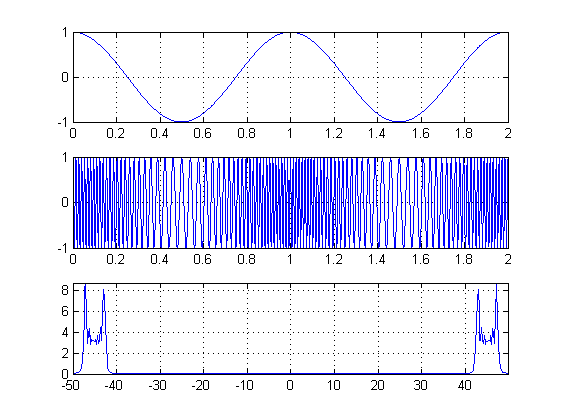
\includegraphics[width=150mm, scale = 0.9]{8_1}\newline
рис. 50. Частотная модуляция сигнала\newline
\end{center}
\end{figure}
\begin{figure}
\begin{center}
\includegraphics[width=150mm, scale = 0.9]{8_2}\newline
рис. 51. Фазовая модуляция сигнала\newline
\end{center}
\end{figure}
Смоделируем ход работы в среде simulink
\begin{figure}
\begin{center}
\includegraphics[width=150mm, scale = 0.9]{8_3}\newline
рис. 52. Модель для частотной модуляции\newline
\end{center}
\end{figure}
\begin{figure}
\begin{center}
\includegraphics[width=150mm, scale = 0.9]{8_4}\newline
рис. 53. Исходный сигнал\newline
\end{center}
\end{figure}
\begin{figure}
\begin{center}
\includegraphics[width=150mm, scale = 0.9]{8_5}\newline
рис. 54. Моделированный сигнал\newline
\end{center}
\end{figure}
\begin{figure}
\begin{center}
\includegraphics[width=150mm, scale = 0.9]{8_6}\newline
рис. 55. Спектр моделированного сигнала\newline
\end{center}
\end{figure}
\begin{figure}
\begin{center}
\includegraphics[width=150mm, scale = 0.9]{8_7}\newline
рис. 56. Модель для фазовой модуляции\newline
\end{center}
\end{figure}
\begin{figure}
\begin{center}
\includegraphics[width=150mm, scale = 0.9]{8_8}\newline
рис. 57. Исходный сигнал\newline
\end{center}
\end{figure}
\begin{figure}
\begin{center}
\includegraphics[width=150mm, scale = 0.9]{8_9}\newline
рис. 58. Моделированный сигнал\newline
\end{center}
\end{figure}
\begin{figure}
\begin{center}
\includegraphics[width=150mm, scale = 0.9]{8_10}\newline
рис. 59. Спектр моделированного сигнала\newline
\end{center}
\end{figure}
Выполним демодуляцию, в том числе с помощью блока захвата фазы (фазовой автоподстройки частоты) Phase-Locked Loop.
\begin{figure}
\begin{center}
\includegraphics[width=150mm, scale = 0.9]{8_11}\newline
рис. 60. Модель фазовой автоподстройки часоты в режиме слежения\newline
\end{center}
\end{figure}
\begin{figure}
\begin{center}
\includegraphics[width=150mm, scale = 0.9]{8_12}\newline
рис. 61. Модель фазовой автоподстройки часоты в режиме захвата и удержания сигнала\newline
\end{center}
\end{figure}
\begin{figure}
\begin{center}
\includegraphics[width=150mm, scale = 0.9]{8_13}\newline
рис. 62. Исходный сигнал\newline
\end{center}
\end{figure}
\begin{figure}
\begin{center}
\includegraphics[width=150mm, scale = 0.9]{8_14}\newline
рис. 63. Моделированный сигнал\newline
\end{center}
\end{figure}
\begin{figure}
\begin{center}
\includegraphics[width=150mm, scale = 0.9]{8_15}\newline
рис. 64. Сигнал на выходе ФНЧ\newline
\end{center}
\end{figure}
\begin{figure}
\begin{center}
\includegraphics[width=150mm, scale = 0.9]{8_16}\newline
рис. 66. Сигнал на выходе фазового детектора\newline
\end{center}
\end{figure}
\begin{figure}
\begin{center}
\includegraphics[width=150mm, scale = 0.9]{8_17}\newline
рис. 67. Сигнал на выходе ГУН\newline
\end{center}
\end{figure}
\section{Вывод}
Различие между фазовой и частотной модуляцией обнаруживается при модуляции спектром частот. При фазовой модуляции индекс модуляции не зависит от частоты модуляции ( т =const), а девиация частоты пропорциональна частоте модуляции (Dw=mW). При частотной модуляции девиация частоты не зависит от частоты модуляции (Dw=const) , а индекс модуляции обратно пропорционален частоте модуляции m=Dw/W.
Частотную и фазовую модуляцию объединяют под общим названием угловой модуляции (УМ). По форме колебаний с угловой модуляцией невозможно определить, к какому виду модуляции относится данное колебание, к ФМ или ЧМ, а при достаточно гладких функциях s(t) формы сигналов ФМ и ЧМ вообще практически не отличаются.
Угловая модуляция, а особенно ЧМ (частотная модуляция), имеет преимущество перед АМ в 
отношении помехозащищенности (т.к. изменение амплтуды из-за шумов можно легко исключить, ограничив амплитуду перед демодуляцией).
\chapter{Лабораторная работа №9}
\section{Постановка задачи}
\begin{enumerate}
\item 
Получить сигналы BPSK, PSK, OQPSK, genQAM, MSK, M-FSK модуляторов.
\item
Построить их сигналы
\item
Провестисравнение изученных методов модуляции цифровых сигналов.
\end{enumerate}
\section{Теоритечиская часть}
Сущность цифровой модуляции заключается в том, что передаваемый непрерывный сигнал дискретизируется во времени, квантуется по уровню и полученные отчеты, следующие в дискретные моменты времени, преобразуются в кодовые комбинации. Полученной последовательностью кодовых видеосигналов модулируется высокочастотный сигнал-переносчик.
Существует 3 основных вида манипуляции сигналов: амплитудная (Amplitude-shift keying (ASK)), частотная (Frequency-shift keying (FSK)) и фазовая (Phase-shift keying (PSK)). Этот набор манипуляций определяется основными характеристиками, которыми обладает любой сигнал. Для моделирования модуляции цифрового сигнала в ходе лаботаторной работы предлагается использовать следующий набор функций:
\begin{enumerate}
\item Функция randerr предназначена для формирования ошибок в цифровом сигнале. Она дает матрицу, в каждой строке которой имеется заданное число случайно расположенных ненулевых элементов.
\item Для оценки помехоустойчивости системы связи необходимо произвести сравнение исходного (передаваемого) сообщения с сообщением, полученным в результате приема, и определить число ошибок, возникших в процессе передачи, а также вероятность ошибки. Эти действия выполняются функциями symerr и biterr, первая из которых подсчитывает число несовпадающих символах в двух сообщениях, а вторая — число несовпадающих битов в двоичных представлениях этих символов. Кроме числа ошибок, обе функции могут возвращать долю ошибок в общем числе символов (битов) и индикаторы мест возникновения ошибок.
\item Последние две функции данной группы предназначены для графического отображения сигналов с квадратурной манипуляцией. Функция eyediagram выводит так называемую глазковую диаграмму, а функция scatterplot — диаграмму рассеяния.
\end{enumerate}
\begin{enumerate}
\item Амплитудная манипуляция (ASK) — изменение сигнала, при котором скачкообразно меняется амплитуда несущего колебания. АМн можно рассматривать как частный случай квадратурной манипуляции.
\item При частотной манипуляции (FSK) значениям «0» и «1» информационной последовательности соответствуют определённые частоты синусоидального сигнала при неизменной амплитуде. Частотная манипуляция весьма помехоустойчива. Однако при частотной манипуляции неэкономно расходуется ресурс полосы частот телефонного канала. Поэтому этот вид модуляции применяется в низкоскоростных протоколах, позволяющих осуществлять связь по каналам с низким отношением сигнал/шум.
\item Минимальная частотная модуляция (MSK) представляет собой способ модуляции, при котором не происходит скачков фазы и изменение частоты происходит в моменты пересечения несущей нулевого уровня. MSK уникальна потому, что значение частот соответствующих логическим «0» и «1» отличаются на величину равную половине скорости передачи данных.
\item Фазовая манипуляция (PSK) — один из видов фазовой модуляции, при которой фаза несущего колебания меняется скачкообразно в зависимости от информационного сообщения.
\item Квадратурной амплитудной манипуляцией (QASK) называется манипуляция, при которой изменяется как фаза, так и амплитуда сигнала, что позволяет увеличить количество информации, передаваемой одним состоянием (отсчётом) сигнала. 
\end{enumerate}
\section{Код matlab}
\begin{verbatim}
%BPSK modulation
h = modem.pskmod('M', 2);
g = modem.pskdemod('M', 2);
msg = randint(10,1,2);
modSignal = modulate(h,msg);
errSignal = (randerr(1,10, 3) ./ 30)';
modSignal = modSignal + errSignal;
demodSignal = demodulate(g,modSignal);
scatterplot(modSignal);
eyediagram(modSignal,10);
scatterplot(demodSignal);
eyediagram(demodSignal,10);

%PSK modulation
h = modem.pskmod('M', 8);
g = modem.pskdemod('M', 8);
msg = randint(10,1,8);
modSignal = modulate(h,msg);
errSignal = (randerr(1,10, 3) ./ 30)';
modSignal = modSignal + errSignal;
demodSignal = demodulate(g,modSignal);
scatterplot(modSignal);
eyediagram(modSignal,10);
scatterplot(demodSignal);
eyediagram(demodSignal,10);

%OQPSK modulation
h = modem.oqpskmod;
g = modem.oqpskdemod;
msg = randint(200,1,4);
modSignal = modulate(h,msg);
errSignal = (randerr(1,400, 100) ./ 30)';
modSignal = modSignal + errSignal;
demodSignal = demodulate(g,modSignal);
scatterplot(modSignal);
eyediagram(modSignal,10);
scatterplot(demodSignal);
eyediagram(demodSignal,10);

%GENQAM modulation
M = 5;
h = modem.genqammod('Constellation', exp(1i*2*pi*[0:M-1]/M));
g = modem.genqamdemod('Constellation', exp(1i*2*pi*[0:M-1]/M));
msg = randint(10,1,8);
modSignal = modulate(h,msg);
errSignal = (randerr(1,10, 3) ./ 30)';
modSignal = modSignal + errSignal;
demodSignal = demodulate(g,modSignal);
scatterplot(modSignal);
eyediagram(modSignal,10);
scatterplot(demodSignal);
eyediagram(demodSignal,10);

%MSK modulation
h = modem.mskmod('SamplesPerSymbol', 10);
g = modem.mskdemod('SamplesPerSymbol', 10);
msg = randint(10,1,2);
modSignal = modulate(h, msg);
errSignal = (randerr(1,100, 3) ./ 30)';
modSignal = modSignal + errSignal;
demodSignal = demodulate(g, modSignal);
scatterplot(modSignal);
eyediagram(modSignal,10);
scatterplot(demodSignal);
eyediagram(demodSignal,10);
\end{verbatim}
\section{Результаты работы}
\begin{figure}
\begin{center}
\includegraphics[width=150mm, scale = 0.9]{9_1}\newline
рис. 68. Сигнальное созвездие BPSK-модуляции\newline
\end{center}
\end{figure}
\begin{figure}
\begin{center}
\includegraphics[width=150mm, scale = 0.9]{9_2}\newline
рис. 69. Глазковая диаграмма BPSK-модуляции\newline
\end{center}
\end{figure}
\begin{figure}
\begin{center}
\includegraphics[width=150mm, scale = 0.9]{9_3}\newline
рис. 70. Сигнальное созвездие BPSK-демодуляции\newline
\end{center}
\end{figure}
\begin{figure}
\begin{center}
\includegraphics[width=150mm, scale = 0.9]{9_4}\newline
рис. 71. Глазковая диаграмма BPSK-демодуляции\newline
\end{center}
\end{figure}
\begin{figure}
\begin{center}
\includegraphics[width=150mm, scale = 0.9]{9_5}\newline
рис. 72. Сигнальное созвездие PSK-модуляции\newline
\end{center}
\end{figure}
\begin{figure}
\begin{center}
\includegraphics[width=150mm, scale = 0.9]{9_6}\newline
рис. 73. Глазковая диаграмма PSK-модуляции\newline
\end{center}
\end{figure}
\begin{figure}
\begin{center}
\includegraphics[width=150mm, scale = 0.9]{9_7}\newline
рис. 74. Сигнальное созвездие PSK-демодуляции\newline
\end{center}
\end{figure}
\begin{figure}
\begin{center}
\includegraphics[width=150mm, scale = 0.9]{9_8}\newline
рис. 75. Глазковая диаграмма PSK-демодуляции\newline
\end{center}
\end{figure}
\begin{figure}
\begin{center}
\includegraphics[width=150mm, scale = 0.9]{9_9}\newline
рис. 76. Сигнальное созвездие OQPSK-модуляции\newline
\end{center}
\end{figure}
\begin{figure}
\begin{center}
\includegraphics[width=150mm, scale = 0.9]{9_10}\newline
рис. 77. Глазковая диаграмма OQPSK-модуляции\newline
\end{center}
\end{figure}
\begin{figure}
\begin{center}
\includegraphics[width=150mm, scale = 0.9]{9_11}\newline
рис. 78. Сигнальное созвездие OQPSK-демодуляции\newline
\end{center}
\end{figure}
\begin{figure}
\begin{center}
\includegraphics[width=150mm, scale = 0.9]{9_12}\newline
рис. 79. Глазковая диаграмма OQPSK-демодуляции\newline
\end{center}
\end{figure}
\begin{figure}
\begin{center}
\includegraphics[width=150mm, scale = 0.9]{9_13}\newline
рис. 80. Сигнальное созвездие genQAM-модуляции\newline
\end{center}
\end{figure}
\begin{figure}
\begin{center}
\includegraphics[width=150mm, scale = 0.9]{9_14}\newline
рис. 81. Глазковая диаграмма genQAM-модуляции\newline
\end{center}
\end{figure}
\begin{figure}
\begin{center}
\includegraphics[width=150mm, scale = 0.9]{9_15}\newline
рис. 82. Сигнальное созвездие genQAM-демодуляции\newline
\end{center}
\end{figure}
\begin{figure}
\begin{center}
\includegraphics[width=150mm, scale = 0.9]{9_16}\newline
рис. 83. Глазковая диаграмма genQAM-демодуляции\newline
\end{center}
\end{figure}
\begin{figure}
\begin{center}
\includegraphics[width=150mm, scale = 0.9]{9_17}\newline
рис. 84. Сигнальное созвездие MSK-модуляции\newline
\end{center}
\end{figure}
\begin{figure}
\begin{center}
\includegraphics[width=150mm, scale = 0.9]{9_18}\newline
рис. 82. Глазковая диаграмма MSK-модуляции\newline
\end{center}
\end{figure}
\begin{figure}
\begin{center}
\includegraphics[width=150mm, scale = 0.9]{9_19}\newline
рис. 83. Сигнальное созвездие MSK-демодуляции\newline
\end{center}
\end{figure}
\begin{figure}
\begin{center}
\includegraphics[width=150mm, scale = 0.9]{9_20}\newline
рис. 84. Глазковая диаграмма MSK-демодуляции\newline
\end{center}
\end{figure}
Смоделируем проделаные опыты при помощи simulink
\begin{figure}
\begin{center}
\includegraphics[width=150mm, scale = 0.9]{9_21}\newline
рис. 85. Модель BPSK-модуляции\newline
\end{center}
\end{figure}
\begin{figure}
\begin{center}
\includegraphics[width=150mm, scale = 0.9]{9_22}\newline
рис. 86. Сигнальное созвездие BPSK-модуляции\newline
\end{center}
\end{figure}
\begin{figure}
\begin{center}
\includegraphics[width=150mm, scale = 0.9]{9_23}\newline
рис. 87. Модель PSK-модуляции\newline
\end{center}
\end{figure}
\begin{figure}
\begin{center}
\includegraphics[width=150mm, scale = 0.9]{9_34}\newline
рис. 88. Сигнальное созвездие PSK-модуляции.\newline
\end{center}
\end{figure}
\begin{figure}
\begin{center}
\includegraphics[width=150mm, scale = 0.9]{9_35}\newline
рис. 89. Модель OQPSK-модуляции\newline
\end{center}
\end{figure}
\begin{figure}
\begin{center}
\includegraphics[width=150mm, scale = 0.9]{9_36}\newline
рис. 90. Сигнальное созвездие OQPSK-модуляции.\newline
\end{center}
\end{figure}
\begin{figure}
\begin{center}
\includegraphics[width=150mm, scale = 0.9]{9_37}\newline
рис. 91. Модель genQAM-модуляции\newline
\end{center}
\end{figure}
\begin{figure}
\begin{center}
\includegraphics[width=150mm, scale = 0.9]{9_38}\newline
рис. 92. Сигнальное созвездие genQAM-модуляции\newline
\end{center}
\end{figure}
\begin{figure}
\begin{center}
\includegraphics[width=150mm, scale = 0.9]{9_39}\newline
рис. 93. Модель MSK-модуляции\newline
\end{center}
\end{figure}
\begin{figure}
\begin{center}
\includegraphics[width=150mm, scale = 0.9]{9_40}\newline
рис. 93. Сигнальное созвездие MSK-модуляции.\newline
\end{center}
\end{figure}
\section{Вывод}
Уровень модуляции определяет количество состояний несущей, используемых для передачи информации. Чем выше этот уровень, тем большими скоростными возможностями и меньшей помехоустойчивостью модуляция обладает. Число бит, передаваемых одним состоянием, определяется как $Log N$, где N — уровень модуляции. Таким образом, чем выше уровень модуляции, тем больше данных мы можем передать (или потерять) за единицу времени. Так же уровень модуляции напрямую зависит от приемника сигнала: чем более точный приемник, тем больший уровень модуляции мы можем задать.
\end{document}